\documentclass[10pt,a4paper]{article}%
\usepackage[T1]{fontenc}%
\usepackage[utf8]{inputenc}%
\usepackage{lmodern}%
\usepackage{textcomp}%
\usepackage{lastpage}%
\usepackage{geometry}%
\geometry{top=1.8cm,bottom=3.5cm,left=1cm,right=1cm}%



%

\usepackage[utf8]{inputenc}
\usepackage{geometry}
\usepackage{graphicx}
\usepackage{tikz}
\usepackage{tabularx}
\usepackage{multicol}
\usepackage{multirow}
\usepackage{array,booktabs,ragged2e}
\usepackage{amsmath}
\usepackage{xkeyval}
\usepackage{float}
\usepackage{physics}
\usepackage{tfrupee}
\usepackage{mathtools} %underbrace symbol
\usepackage{adjustbox} 
\usepackage{xcolor}
\usepackage{colortbl}
\usepackage{tkz-euclide}
\usepackage{pgf-pie}
\usepackage[misc]{ifsym} %Used in tally mark
\usetikzlibrary{patterns,calc}

\newcommand{\scalefactor}{1}


\geometry{top=2.5cm, bottom=1.25cm, left=1.5cm, right=1.5cm}
%%%%%%%%%%%%%%%%%%%%%%%%%%%%%%%%%%%%%%colours%%%%%%%%%%%%%%%%%%%%%%%%%%%%%%%%%%%%%%%%%%
\definecolor{Color1}{RGB}{106,168,79}%
\definecolor{Color2}{RGB}{255,136,23}%
\definecolor{Color3}{RGB}{70,189,198}%
\definecolor{Color4}{RGB}{248,201,40}%
\definecolor{Color5}{RGB}{241,55,16}%

%patterncolor
\definecolor{PatternColor1}{RGB}{0,255,0} %green
\definecolor{PatternColor2}{RGB}{255,128,0} %orange
\definecolor{PatternColor3}{RGB}{70,189,198} %sky blue

\definecolor{cellgreen}{rgb}{0.776,0.937,0.808}
\definecolor{cellred}{rgb}{1,0.78,0.808}
\definecolor{hrulecolor1}{RGB}{68,114,196}%
\definecolor{blue}{HTML}{E9EBF5}%

\definecolor{lightcyan}{RGB}{224, 255, 255}   % Light cyan color
\definecolor{lightpink}{RGB}{255, 182, 193}   % Light pink color
\definecolor{lightlavender}{RGB}{230, 230, 250} % Light lavender color
\definecolor{lightblue}{RGB}{173, 216, 230}   % Light blue color

\definecolor{hrulecolor1}{RGB}{68,114,196}%


\definecolor{Highlightred}{RGB}{248, 131, 121} % 172, 225, 175
\definecolor{Highlightgreen}{RGB}{152, 251, 152}
\definecolor{Highlightyellow}{RGB}{251, 236, 93} %0, 240, 168

\newcommand{\highred}[1]{\sethlcolor{Highlightred}\hl{#1}}%below 40 for correct option Only
\newcommand{\highgreen}[1]{\sethlcolor{Highlightgreen}\hl{#1}}%Above 75 for correct option Only
\newcommand{\highyellow}[1]{\sethlcolor{Highlightyellow}\hl{#1}}% In between perctange for correct option Only

\newcommand{\highyellowred}[1]{\sethlcolor{Highlightyellow}\textcolor{red}{\hl{#1}}}

\newcommand{\highno}[1]{{#1}}

\newcommand{\answerkeychaptername}[1]{ 
    \needspace{5\baselineskip}
    \begin{center}
    \medskip
    \Large  \underline{\textbf{#1}}
    \medskip
    \end{center}}


%%%%%%%%%%%%%%%%%%%

\newcommand{\examdetails}[5]{

% 1 - School Name
% 2 - Class section (8A)
% 3 - subject
% 4 - Exam Held Date
% 5 - Exam Tag

\def \schoolname{#1}
\def \classsection{#2}
\def \subject{#3}
\def \examheldon{#4}
\def \schooltag{#5}
}



%%%%%%%%%%%% Index Page Header

\newcommand{\indexpage}{
\fancypagestyle{indexpage}{
\renewcommand{\headrulewidth}{0pt}
\renewcommand{\footrulewidth}{0pt}
\fancyhead{}
\fancyfoot{}
\fancyfoot[L]{}
\fancyhead[L]{
    \renewcommand{\arraystretch}{1}
    \arrayrulecolor{hrulecolor1} 
    \begin{tabular}{m{3cm} m{0.2cm} >{\centering\arraybackslash}m{13cm}}
    
\includegraphics[width=3cm]{logo.png}  & & \LARGE \textbf{\schoolname} \\
    \cline{3-3}
    \small www.learnbasics.fun 
    & & \medskip \Large \textbf{LaPIS Diagnostic Test Report}  \medskip\\
    & & \medskip \Large \textbf{Class\;\classsection\;- \subject} \medskip\\
    \end{tabular}
    }
\renewcommand{\footrulewidth}{0pt}}
}

%%%%%%%%%%% Class Details in Index Page

% 1 - Class Performance
% 2 - Total Student
% 3 - Present
% 4 - Absent

\newcommand{\classdetails}[4]{
\begin{minipage}[c]{0.3\textwidth}
    \begin{center}
    \fbox{\parbox[c]{3.5cm}{\vspace{0.1cm} \centering \textbf{Exam Held On} \\ \vspace{0.1cm} \textbf{\examheldon}\vspace{0.1cm} }}
    \end{center} 
\end{minipage}%
\hfill
\begin{minipage}[c]{0.3\textwidth}
    \begin{center}
    \fbox{\parbox[c]{3.5cm}{\vspace{0.1cm} \centering \textbf{Performance} \\ \vspace{0.1cm} \textbf{#1 \%}\vspace{0.1cm} }}
    \end{center}
\end{minipage}
\hfill
\begin{minipage}[c]{0.3\textwidth}
    \begin{large}
    \begin{center}
    \fbox{\parbox[c]{3.5cm}{\vspace{0.1cm} \centering \textbf{Total Student} \\ \vspace{0.1cm} \textbf{#2}\vspace{0.1cm} }} \\
    \end{center}
    \begin{center}
    \fbox{\parbox[c]{1.8cm}{\vspace{0.1cm} \centering \textbf{Present}\\ \vspace{0.1cm} \textbf{#3}\vspace{0.1cm} }} \hspace{2mm}%
    \fbox{\parbox[c]{1.8cm}{\vspace{0.1cm} \centering \textbf{Absent}\\ \vspace{0.1cm} \textbf{#4}\vspace{0.1cm} }}
    \end{center}
    \end{large}
\end{minipage}}


%%%%%%%%%%%%%%%% Header - Common


\newcommand{\header}[2]{
        \fancypagestyle{header#1}{
        \renewcommand{\headrulewidth}{0pt}
        \renewcommand{\footrulewidth}{0pt}
        \fancyhead{
        }
        \fancyfoot{
        }
        \fancyhead[L]{
        \vspace{0.2cm}
        
\includegraphics[width = 3cm]{logo.png}
        }
        \fancyfoot[L]{
        \vspace{0cm}
        Learn Basics%
        }
        \fancyfoot[C]{
        \vspace{0cm}
        %
        Class \classsection\;-\;\subject\;- Page \thepage %
        }
        \fancyfoot[R]{
        \vspace{0cm}
        LaPIS held on \examheldon%
        }
        \fancyhead[C]{
            \begin{center}
            \Large \textbf{#2}
            \end{center}   
        }
        \renewcommand{\footrulewidth}{1pt}
        }
}


%%%%%%%%%%%%%%%%%%%%%%%%%% Landscape page Template

%%%%%%%%%%%%%%%% Empty Page
\newcommand{\emptypage}[1]{
    \fancypagestyle{emptypage#1}{
    \renewcommand{\headrulewidth}{0pt}
    \renewcommand{\footrulewidth}{0pt}
    \fancyhead{}
    \fancyfoot{}}
}

%%%%%%%%%%%%%%% landScape header

\newcommand{\landscapeheader}[1]{
\begin{minipage}{0.1\linewidth}

\includegraphics[width=3cm]{logo.png}
\end{minipage}
\begin{minipage}{0.8\linewidth}
\begin{center}  
    \begin{large}
        {\Large \textbf{#1}} 
    \end{large}
    \end{center}
\end{minipage}
}


%%%%%%%%%%%%%% Question wise name List 

\newcommand{\namelisttable}[4]{
\renewcommand{\arraystretch}{#1}
\begin{tabular}{|>{\centering \arraybackslash} m{#2cm}|}
\hline
{\textbf{#3}} \\
\hline
\RaggedRight {#4}\\
\hline
\end{tabular}
\vspace{0.2cm}
}

%%%%%%%%%%%%%%%%%%%%%%%%%%%%%%%%%%%%%%%%%%%%%%%%%%%%%%%%%%%

\newcommand{\pagerotate}[1]{
    \KOMAoptions{paper=#1, DIV=last}
    \newgeometry{top=1.8cm,bottom=2cm,left=1cm,right=1cm}%
    \fancyheadoffset{10pt}
}

\newcommand{\greentick}{\textcolor[RGB]{0,128,0}{\ding{52}}}

 \newcommand{\redcross}{\textcolor[RGB]{255,0,0}{\ding{55}}}


 \newcommand\yellowalert[1][2ex]{%
 \scaleto{\stackengine{0.3pt}{\scalebox{1.1}[.9]{%
 \color{yellow}$\blacktriangle$}}{\tiny\bfseries !}{O}{c}{F}{F}{L}}{#1}%
 }

\newcommand{\topicperformancenote}{
\bigskip
\centering
\begin{tabular}{|c|c|c|c|c|c|}
\hline
\cellcolor{cellgreen} \greentick  & Performance Between 75\% and 100\%  & 
\yellowalert  & Performance Between 40\% and 75\%  &
\redcross  & Performance Between 0\% and 40\%   
\\
\hline 
\end{tabular}
}

\newcommand{\consolidatedmarknote}{
% \vspace{0.51cm}
\hspace{1cm}
\parbox[c]{15cm}{\vspace{0.1cm}
\textbf{Note:}\\
We have provided an extra option called \textbf{Learn Later} as \textbf{Option E} which students can select if they are unsure of an answer to a question.}}
\makeatletter




\define@key{maimgleftFourOne}{myanswerquestion}{\def\maimgleftFourOnemyanswerquestion{#1}} 
\define@key{maimgleftFourOne}{myanswercontent}{\def\maimgleftFourOnemyanswercontent{#1}} 


\define@key{maimgleftFourOne}{questionnumber}{\def\maimgleftFourOnequestionnumber{#1}} 
\define@key{maimgleftFourOne}{questiontext}{\def\maimgleftFourOnequestiontext{#1}}
\define@key{maimgleftFourOne}{imgtabletikz}{\def\maimgtabletikz{#1}}
\define@key{maimgleftFourOne}{optionA}{\def\maimgleftFourOneoptionA{#1}}
\define@key{maimgleftFourOne}{optionB}{\def\maimgleftFourOneoptionB{#1}}
\define@key{maimgleftFourOne}{optionC}{\def\maimgleftFourOneoptionC{#1}}
\define@key{maimgleftFourOne}{optionD}{\def\maimgleftFourOneoptionD{#1}}
\define@key{maimgleftFourOne}{questionTag}{\def\maimgleftFourOnequestionTag{#1}} 
\define@key{maimgleftFourOne}{correctoption}{\def\maimgleftFourOnecorrectoption{#1}}
\define@key{maimgleftFourOne}{leftmini}{\def\maimgleftFourOneleftmini{#1}}
\define@key{maimgleftFourOne}{rightmini}{\def\maimgleftFourOnerightmini{#1}}

% COMMAND FOR maimgleftFourOne 

\newcommand{\maimgleftFourOne}[1]{%
\setkeys{maimgleftFourOne}{#1}%



\begin{raggedright}
\textbf{Question \maimgleftFourOnequestionnumber:} 
\maimgleftFourOnemyanswerquestion\\
\centering
\begin{qanswerbox}
\centering
\maimgleftFourOnemyanswercontent
\end{qanswerbox}
\RaggedRight
\maimgleftFourOnequestiontext\\
\medskip
\end{raggedright}
\begin{minipage}[]{\maimgleftFourOneleftmini\linewidth}
\Centering
\maimgtabletikz 
\end{minipage}\hfill
\begin{minipage}[]{\maimgleftFourOnerightmini\linewidth}
  (a) \medskip \maimgleftFourOneoptionA\\
  (b) \medskip \maimgleftFourOneoptionB\\
  (c) \medskip \maimgleftFourOneoptionC\\
  (d) \medskip \maimgleftFourOneoptionD\\  
\end{minipage}
}



%-----------------------------------------------------------
         % My answer text bottom 4 option in 1 row
%-----------------------------------------------------------

% Define key FOR matextbottomOneFour

\define@key{matextbottomOneFour}{myanswerquestion}{\def\matextbottomOneFourmyanswerquestion{#1}} 
\define@key{matextbottomOneFour}{myanswercontent}{\def\matextbottomOneFourmyanswercontent{#1}} 

\define@key{matextbottomOneFour}{questionnumber}{\def\matextbottomOneFourquestion{#1}}
\define@key{matextbottomOneFour}{questiontext}{\def\matextbottomOneFourquestiontext{#1}}
\define@key{matextbottomOneFour}{optionA}{\def\matextbottomOneFouroptionA{#1}}
\define@key{matextbottomOneFour}{optionB}{\def\matextbottomOneFouroptionB{#1}}
\define@key{matextbottomOneFour}{optionC}{\def\matextbottomOneFouroptionC{#1}}
\define@key{matextbottomOneFour}{optionD}{\def\matextbottomOneFouroptionD{#1}}
\define@key{matextbottomOneFour}{questionTag}{\def\matextbottomOneFourquestionTag{#1}}
\define@key{matextbottomOneFour}{correctoption}{\def\matextbottomOneFourcorrectoption{#1}}

% COMMAND FOR matextbottomOneFour %

\newcommand{\matextbottomOneFour}[1]{%
\setkeys{matextbottomOneFour}{#1}%



\begin{raggedright}
\textbf{Question \matextbottomOneFourquestion:} 
\matextbottomOneFourmyanswerquestion\\
\centering
% \workspace{abc}
\begin{qanswerbox}
\centering
\matextbottomOneFourmyanswercontent
\end{qanswerbox}
\RaggedRight
\matextbottomOneFourquestiontext\\
\RaggedRight
\begin{multicols}{4}
  (a) \medskip \matextbottomOneFouroptionA\\
  (b) \medskip \matextbottomOneFouroptionB\\
  (c) \medskip \matextbottomOneFouroptionC\\
  (d) \medskip \matextbottomOneFouroptionD\\
\end{multicols}
\end{raggedright}
}

%-----------------------------------------------------------
         % My answer text bottom 4 option in 2 row
%-----------------------------------------------------------

% Define key FOR matextbottomTwoTwo

\define@key{matextbottomTwoTwo}{myanswerquestion}{\def\matextbottomTwoTwomyanswerquestion{#1}} 
\define@key{matextbottomTwoTwo}{myanswercontent}{\def\matextbottomTwoTwomyanswercontent{#1}} 

\define@key{matextbottomTwoTwo}{questionnumber}{\def\matextbottomTwoTwoquestion{#1}}
\define@key{matextbottomTwoTwo}{questiontext}{\def\matextbottomTwoTwoquestiontext{#1}}
\define@key{matextbottomTwoTwo}{optionA}{\def\matextbottomTwoTwooptionA{#1}}
\define@key{matextbottomTwoTwo}{optionB}{\def\matextbottomTwoTwooptionB{#1}}
\define@key{matextbottomTwoTwo}{optionC}{\def\matextbottomTwoTwooptionC{#1}}
\define@key{matextbottomTwoTwo}{optionD}{\def\matextbottomTwoTwooptionD{#1}}
\define@key{matextbottomTwoTwo}{questionTag}{\def\matextbottomTwoTwoquestionTag{#1}}
\define@key{matextbottomTwoTwo}{correctoption}{\def\matextbottomTwoTwocorrectoption{#1}}

% COMMAND FOR matextbottomTwoTwo %

\newcommand{\matextbottomTwoTwo}[1]{%
\setkeys{matextbottomTwoTwo}{#1}%



\begin{raggedright}
\textbf{Question \matextbottomTwoTwoquestion:} 
\matextbottomTwoTwomyanswerquestion\\
\centering
% \workspace{abc}
\begin{qanswerbox}
\centering
\matextbottomTwoTwomyanswercontent
\end{qanswerbox}
\RaggedRight
\matextbottomTwoTwoquestiontext\\
\RaggedRight
\begin{multicols}{2}
  (a) \medskip \matextbottomTwoTwooptionA\\
  (c) \medskip \matextbottomTwoTwooptionC\\
  \columnbreak
  (b) \medskip \matextbottomTwoTwooptionB\\
  (d) \medskip \matextbottomTwoTwooptionD\\
\end{multicols}
\end{raggedright}
}


%-----------------------------------------------------------
         % My answer text bottom 4 option in 1 row
%-----------------------------------------------------------

% Define key FOR matextbottomFourOne

\define@key{matextbottomFourOne}{myanswerquestion}{\def\matextbottomFourOnemyanswerquestion{#1}} 
\define@key{matextbottomFourOne}{myanswercontent}{\def\matextbottomFourOnemyanswercontent{#1}} 

\define@key{matextbottomFourOne}{questionnumber}{\def\matextbottomFourOnequestion{#1}}
\define@key{matextbottomFourOne}{questiontext}{\def\matextbottomFourOnequestiontext{#1}}
\define@key{matextbottomFourOne}{optionA}{\def\matextbottomFourOneoptionA{#1}}
\define@key{matextbottomFourOne}{optionB}{\def\matextbottomFourOneoptionB{#1}}
\define@key{matextbottomFourOne}{optionC}{\def\matextbottomFourOneoptionC{#1}}
\define@key{matextbottomFourOne}{optionD}{\def\matextbottomFourOneoptionD{#1}}
\define@key{matextbottomFourOne}{questionTag}{\def\matextbottomFourOnequestionTag{#1}}
\define@key{matextbottomFourOne}{correctoption}{\def\matextbottomFourOnecorrectoption{#1}}

% COMMAND FOR matextbottomFourOne %

\newcommand{\matextbottomFourOne}[1]{%
\setkeys{matextbottomFourOne}{#1}%



\begin{raggedright}
\textbf{Question \matextbottomFourOnequestion:} 
\matextbottomFourOnemyanswerquestion\\
\centering
% \workspace{abc}
\begin{qanswerbox}
\centering
\matextbottomFourOnemyanswercontent
\end{qanswerbox}
\RaggedRight
\matextbottomFourOnequestiontext\\
\RaggedRight
  (a) \medskip \matextbottomFourOneoptionA\\
  (b) \medskip \matextbottomFourOneoptionB\\
  (c) \medskip \matextbottomFourOneoptionC\\
  (d) \medskip \matextbottomFourOneoptionD\\
\end{raggedright}
}

%-----------------------------------------------------------
         % My answer image bottom 4 option in 1 row
%-----------------------------------------------------------

% Define key FOR maimgbottomOneFour
\define@key{maimgbottomOneFour}{myanswerquestion}{\def\maimgbottomOneFourmyanswerquestion{#1}} 
\define@key{maimgbottomOneFour}{myanswercontent}{\def\maimgbottomOneFourmyanswercontent{#1}} 

\define@key{maimgbottomOneFour}{questionnumber}{\def\maimgbottomOneFourquestionnumber{#1}}
\define@key{maimgbottomOneFour}{questionTag}{\def\maimgbottomOneFourquestionTag{#1}}
\define@key{maimgbottomOneFour}{questiontext}{\def\maimgbottomOneFourquestiontext{#1}}
\define@key{maimgbottomOneFour}{optionA}{\def\maimgbottomOneFouroptionA{#1}}
\define@key{maimgbottomOneFour}{optionB}{\def\maimgbottomOneFouroptionB{#1}}
\define@key{maimgbottomOneFour}{optionC}{\def\maimgbottomOneFouroptionC{#1}}
\define@key{maimgbottomOneFour}{optionD}{\def\maimgbottomOneFouroptionD{#1}}
\define@key{maimgbottomOneFour}{correctoption}{\def\maimgbottomOneFourcorrectoption{#1}}

% COMMAND FOR maimgbottomOneFour %

\newcommand{\maimgbottomOneFour}[1]{%
\setkeys{maimgbottomOneFour}{#1}%



\begin{raggedright}
\textbf{Question \maimgbottomOneFourquestionnumber:} 
\maimgbottomOneFourmyanswerquestion\\
\centering
\begin{qanswerbox}
\centering
\maimgbottomOneFourmyanswercontent
\end{qanswerbox}
\RaggedRight
\maimgbottomOneFourquestiontext 
\begin{multicols}{4}
  (a) {\adjustbox{scale=\scalefactor}{\includegraphics[width=2.5cm, height=2cm]{\maimgbottomOneFouroptionA}}}  \\
  (b) {\adjustbox{scale=\scalefactor}{\includegraphics[width=2.5cm, height=2cm]{\maimgbottomOneFouroptionB}}}   \\
  (c) {\adjustbox{scale=\scalefactor}{\includegraphics[width=2.5cm, height=2cm]{\maimgbottomOneFouroptionC}}}  \\
  (d) {\adjustbox{scale=\scalefactor}{\includegraphics[width=2.5cm, height=2cm]{\maimgbottomOneFouroptionD}}} 
\end{multicols}
\end{raggedright}
}

%-----------------------------------------------------------
             % text bottom 4 option in 1 row
%-----------------------------------------------------------

 \define@key{mcqtextbottomFourOne}{questionnumber}{\def\mcqtextbottomFourOnequestionnumber{#1}} 
 \define@key{mcqtextbottomFourOne}{questionTag}{\def\mcqtextbottomFourOnequestionTag{#1}}
\define@key{mcqtextbottomFourOne}{questiontext}{\def\mcqtextbottomFourOnequestiontext{#1}}
\define@key{mcqtextbottomFourOne}{optionA}{\def\mcqtextbottomFourOneoptionA{#1}}
\define@key{mcqtextbottomFourOne}{optionB}{\def\mcqtextbottomFourOneoptionB{#1}}
\define@key{mcqtextbottomFourOne}{optionC}{\def\mcqtextbottomFourOneoptionC{#1}}
\define@key{mcqtextbottomFourOne}{optionD}{\def\mcqtextbottomFourOneoptionD{#1}}
\define@key{mcqtextbottomFourOne}{correctoption}{\def\mcqtextbottomFourOnecorrectoption{#1}}


\newcommand{\mcqtextbottomFourOne}[1]{%
  \setkeys{mcqtextbottomFourOne}{#1}%


  
  \begin{raggedright}
    \textbf{Question \mcqtextbottomFourOnequestionnumber:} \mcqtextbottomFourOnequestiontext \\
    \medskip
      (a) \medskip \mcqtextbottomFourOneoptionA\\
      (b) \medskip \mcqtextbottomFourOneoptionB\\      
      (c) \medskip \mcqtextbottomFourOneoptionC\\
      (d) \medskip \mcqtextbottomFourOneoptionD\\
   \end{raggedright}
}

%-----------------------------------------------------------

%-----------------------------------------------------------

% DEFINE KEY FOR mcqtextbottomOneFour %

\define@key{mcqtextbottomOneFour}{questionnumber}{\def\mcqtextbottomOneFourquestionnumber{#1}} 
\define@key{mcqtextbottomOneFour}{questiontext}{\def\mcqtextbottomOneFourquestiontext{#1}}
\define@key{mcqtextbottomOneFour}{optionA}{\def\mcqtextbottomOneFouroptionA{#1}}
\define@key{mcqtextbottomOneFour}{optionB}{\def\mcqtextbottomOneFouroptionB{#1}}
\define@key{mcqtextbottomOneFour}{optionC}{\def\mcqtextbottomOneFouroptionC{#1}}
\define@key{mcqtextbottomOneFour}{optionD}{\def\mcqtextbottomOneFouroptionD{#1}}
\define@key{mcqtextbottomOneFour}{questionTag}{\def\mcqtextbottomOneFourquestionTag{#1}} 
\define@key{mcqtextbottomOneFour}{correctoption}{\def\mcqtextbottomOneFourcorrectoption{#1}}

% COMMAND FOR mcqtextbottomOneFour %

\newcommand{\mcqtextbottomOneFour}[1]{%
  \setkeys{mcqtextbottomOneFour}{#1}%


  
  \begin{raggedright}
    \textbf{Question \mcqtextbottomOneFourquestionnumber:} \mcqtextbottomOneFourquestiontext
    \begin{multicols}{4}
      (a) \medskip \mcqtextbottomOneFouroptionA\\
      (b) \medskip \mcqtextbottomOneFouroptionB\\      
      (c) \medskip \mcqtextbottomOneFouroptionC\\
      (d) \medskip \mcqtextbottomOneFouroptionD\\
    \end{multicols}
  \end{raggedright}
}

%-----------------------------------------------------------

%-----------------------------------------------------------

% Define key FOR mcqtextbottomOneTwo 

\define@key{mcqtextbottomOneTwo}{questionnumber}{\def\mcqtextbottomOneTwoquestion{#1}}
\define@key{mcqtextbottomOneTwo}{questiontext}{\def\mcqtextbottomOneTwoquestiontext{#1}}
\define@key{mcqtextbottomOneTwo}{optionA}{\def\mcqtextbottomOneTwooptionA{#1}}
\define@key{mcqtextbottomOneTwo}{optionB}{\def\mcqtextbottomOneTwooptionB{#1}}
\define@key{mcqtextbottomOneTwo}{questionTag}{\def\mcqtextbottomOneTwoquestionTag{#1}}
\define@key{mcqtextbottomOneTwo}{correctoption}{\def\mcqtextbottomOneTwocorrectoption{#1}}

% COMMAND FOR mcqtextbottomOneTwo %

\newcommand{\mcqtextbottomOneTwo}[1]{%
  \setkeys{mcqtextbottomOneTwo}{#1}%


  
  \begin{raggedright}
    \textbf{Question \mcqtextbottomOneTwoquestion:} \mcqtextbottomOneTwoquestiontext\\
    \begin{multicols}{2}
      (a) \medskip \mcqtextbottomOneTwooptionA\\
      (b) \medskip \mcqtextbottomOneTwooptionB\\
    \end{multicols}
  \end{raggedright}
}

%-----------------------------------------------------------

%-----------------------------------------------------------

% Define key FOR mcqtextbottomTwoTwo

\define@key{mcqtextbottomTwoTwo}{questionnumber}{\def\mcqtextbottomTwoTwoquestion{#1}}
\define@key{mcqtextbottomTwoTwo}{questiontext}{\def\mcqtextbottomTwoTwoquestiontext{#1}}
\define@key{mcqtextbottomTwoTwo}{optionA}{\def\mcqtextbottomTwoTwooptionA{#1}}
\define@key{mcqtextbottomTwoTwo}{optionB}{\def\mcqtextbottomTwoTwooptionB{#1}}
\define@key{mcqtextbottomTwoTwo}{optionC}{\def\mcqtextbottomTwoTwooptionC{#1}}
\define@key{mcqtextbottomTwoTwo}{optionD}{\def\mcqtextbottomTwoTwooptionD{#1}}
\define@key{mcqtextbottomTwoTwo}{questionTag}{\def\mcqtextbottomTwoTwoquestionTag{#1}}
\define@key{mcqtextbottomTwoTwo}{correctoption}{\def\mcqtextbottomTwoTwocorrectoption{#1}}

% COMMAND FOR mcqtextbottomTwoTwo %

\newcommand{\mcqtextbottomTwoTwo}[1]{%
  \setkeys{mcqtextbottomTwoTwo}{#1}%


  
  \begin{raggedright}
    \textbf{Question \mcqtextbottomTwoTwoquestion:} \mcqtextbottomTwoTwoquestiontext\\
    \begin{multicols}{2}
      (a) \medskip \mcqtextbottomTwoTwooptionA\\
      (c) \medskip \mcqtextbottomTwoTwooptionC\\
      \columnbreak
      (b) \medskip \mcqtextbottomTwoTwooptionB\\
      (d) \medskip \mcqtextbottomTwoTwooptionD\\
    \end{multicols}
  \end{raggedright}
}

%-----------------------------------------------------------

%-----------------------------------------------------------

% Define key FOR mcqtextsideFourOne


\define@key{mcqtextsideFourOne}{questionnumber}{\def\mcqtextsideFourOnequestionnumber{#1}} 
\define@key{mcqtextsideFourOne}{questionTag}{\def\mcqtextsideFourOnequestionTag{#1}} 
\define@key{mcqtextsideFourOne}{questiontext}{\def\mcqtextsideFourOnequestiontext{#1}}
\define@key{mcqtextsideFourOne}{optionA}{\def\mcqtextsideFourOneoptionA{#1}}
\define@key{mcqtextsideFourOne}{optionB}{\def\mcqtextsideFourOneoptionB{#1}}
\define@key{mcqtextsideFourOne}{optionC}{\def\mcqtextsideFourOneoptionC{#1}}
\define@key{mcqtextsideFourOne}{optionD}{\def\mcqtextsideFourOneoptionD{#1}}
\define@key{mcqtextsideFourOne}{correctoption}{\def\mcqtextsideFourOnecorrectoption{#1}}
\define@key{mcqtextsideFourOne}{leftmini}{\def\mcqtextsideFourOneleftmini{#1}}
\define@key{mcqtextsideFourOne}{rightmini}{\def\mcqtextsideFourOnerightmini{#1}}

% COMMAND FOR mcqtextsideFourOne

\newcommand{\mcqtextsideFourOne}[1]{%
  \setkeys{mcqtextsideFourOne}{#1}%


  
  \begin{raggedright}
  \begin{minipage}[t]{\mcqtextsideFourOneleftmini\linewidth}
    \textbf{Question \mcqtextsideFourOnequestionnumber:} \mcqtextsideFourOnequestiontext\\
  \end{minipage}\hfill
  \begin{minipage}[t]{\mcqtextsideFourOnerightmini\linewidth}
        (a) \medskip \mcqtextsideFourOneoptionA\\
        (b) \medskip \mcqtextsideFourOneoptionB\\
        (c) \medskip \mcqtextsideFourOneoptionC\\
        (d) \medskip \mcqtextsideFourOneoptionD\\
     \end{minipage}
   \end{raggedright}
}

%-----------------------------------------------------------

%-----------------------------------------------------------

% Define key FOR mcqimgbottomOneFour

\define@key{mcqimgbottomOneFour}{questionnumber}{\def\mcqimgbottomOneFourquestionnumber{#1}}
\define@key{mcqimgbottomOneFour}{questionTag}{\def\mcqimgbottomOneFourquestionTag{#1}}
\define@key{mcqimgbottomOneFour}{questiontext}{\def\mcqimgbottomOneFourquestiontext{#1}}
\define@key{mcqimgbottomOneFour}{optionA}{\def\mcqimgbottomOneFouroptionA{#1}}
\define@key{mcqimgbottomOneFour}{optionB}{\def\mcqimgbottomOneFouroptionB{#1}}
\define@key{mcqimgbottomOneFour}{optionC}{\def\mcqimgbottomOneFouroptionC{#1}}
\define@key{mcqimgbottomOneFour}{optionD}{\def\mcqimgbottomOneFouroptionD{#1}}
\define@key{mcqimgbottomOneFour}{correctoption}{\def\mcqimgbottomOneFourcorrectoption{#1}}

% COMMAND FOR mcqimgbottomOneFour %

\newcommand{\mcqimgbottomOneFour}[1]{%
  \setkeys{mcqimgbottomOneFour}{#1}%


  
  \begin{raggedright}
    \textbf{Question \mcqimgbottomOneFourquestionnumber:} \mcqimgbottomOneFourquestiontext \\
    \begin{multicols}{4}
      (a) {\adjustbox{scale=\scalefactor}{\includegraphics[width=2.5cm, height=2cm]{\mcqimgbottomOneFouroptionA}}}  \\
      (b) {\adjustbox{scale=\scalefactor}{\includegraphics[width=2.5cm, height=2cm]{\mcqimgbottomOneFouroptionB}}}   \\
      (c) {\adjustbox{scale=\scalefactor}{\includegraphics[width=2.5cm, height=2cm]{\mcqimgbottomOneFouroptionC}}}  \\
      (d) {\adjustbox{scale=\scalefactor}{\includegraphics[width=2.5cm, height=2cm]{\mcqimgbottomOneFouroptionD}}} 
    \end{multicols}
  \end{raggedright}
}

%-----------------------------------------------------------

%-----------------------------------------------------------

% Define key FOR mcqimgdbottomOneFour

\define@key{mcqimgdbottomOneFour}{questionnumber}{\def\mcqimgdbottomOneFourquestionnumber{#1}}
\define@key{mcqimgdbottomOneFour}{questionTag}{\def\mcqimgdbottomOneFourquestionTag{#1}}
\define@key{mcqimgdbottomOneFour}{questiontext}{\def\mcqimgdbottomOneFourquestiontext{#1}}
\define@key{mcqimgdbottomOneFour}{optionA}{\def\mcqimgdbottomOneFouroptionA{#1}}
\define@key{mcqimgdbottomOneFour}{optionAtext}{\def\mcqimgdbottomOneFouroptionAtext{#1}}
\define@key{mcqimgdbottomOneFour}{optionB}{\def\mcqimgdbottomOneFouroptionB{#1}}
\define@key{mcqimgdbottomOneFour}{optionBtext}{\def\mcqimgdbottomOneFouroptionBtext{#1}}
\define@key{mcqimgdbottomOneFour}{optionC}{\def\mcqimgdbottomOneFouroptionC{#1}}
\define@key{mcqimgdbottomOneFour}{optionCtext}{\def\mcqimgdbottomOneFouroptionCtext{#1}}
\define@key{mcqimgdbottomOneFour}{optionD}{\def\mcqimgdbottomOneFouroptionD{#1}}
\define@key{mcqimgdbottomOneFour}{optionDtext}{\def\mcqimgdbottomOneFouroptionDtext{#1}}
\define@key{mcqimgdbottomOneFour}{correctoption}{\def\mcqimgdbottomOneFourcorrectoption{#1}}

% COMMAND FOR mcqimgdbottomOneFour %

\newcommand{\mcqimgdbottomOneFour}[1]{%
  \setkeys{mcqimgdbottomOneFour}{#1}%


  
  \begin{raggedright}
    \textbf{Question \mcqimgdbottomOneFourquestionnumber:} \mcqimgdbottomOneFourquestiontext \\
    \begin{multicols}{4}
       {\adjustbox{scale=\scalefactor}{\includegraphics[width=2.5cm, height=2cm]{\mcqimgdbottomOneFouroptionA}}} \\*
      (a) \mcqimgdbottomOneFouroptionAtext \\

       {\adjustbox{scale=\scalefactor}{\includegraphics[width=2.5cm, height=2cm]{\mcqimgdbottomOneFouroptionB}}} \\*      
      (b) \mcqimgdbottomOneFouroptionBtext \\

       {\adjustbox{scale=\scalefactor}{\includegraphics[width=2.5cm, height=2cm]{\mcqimgdbottomOneFouroptionC}}} \\*
      (c) \mcqimgdbottomOneFouroptionCtext \\

       {\adjustbox{scale=\scalefactor}{\includegraphics[width=2.5cm, height=2cm]{\mcqimgdbottomOneFouroptionD}}} \\*
      (d) \mcqimgdbottomOneFouroptionDtext
    \end{multicols}
  \end{raggedright}
  }

%-----------------------------------------------------------

%-----------------------------------------------------------

% Define key FOR mcqimgleftFourOne

\define@key{mcqimgleftFourOne}{questionnumber}{\def\mcqimgleftFourOnequestionnumber{#1}} 
\define@key{mcqimgleftFourOne}{questiontext}{\def\mcqimgleftFourOnequestiontext{#1}}
\define@key{mcqimgleftFourOne}{imgtabletikz}{\def\mcqimgtabletikz{#1}}
\define@key{mcqimgleftFourOne}{optionA}{\def\mcqimgleftFourOneoptionA{#1}}
\define@key{mcqimgleftFourOne}{optionB}{\def\mcqimgleftFourOneoptionB{#1}}
\define@key{mcqimgleftFourOne}{optionC}{\def\mcqimgleftFourOneoptionC{#1}}
\define@key{mcqimgleftFourOne}{optionD}{\def\mcqimgleftFourOneoptionD{#1}}
\define@key{mcqimgleftFourOne}{questionTag}{\def\mcqimgleftFourOnequestionTag{#1}} 
\define@key{mcqimgleftFourOne}{correctoption}{\def\mcqimgleftFourOnecorrectoption{#1}}
\define@key{mcqimgleftFourOne}{leftmini}{\def\mcqimgleftFourOneleftmini{#1}}
\define@key{mcqimgleftFourOne}{rightmini}{\def\mcqimgleftFourOnerightmini{#1}}

% COMMAND FOR mcqimgleftFourOne 

\newcommand{\mcqimgleftFourOne}[1]{%
  \setkeys{mcqimgleftFourOne}{#1}%

  
  \begin{raggedright}
    \textbf{Question \mcqimgleftFourOnequestionnumber:} \mcqimgleftFourOnequestiontext\\
    \medskip
  \end{raggedright}
  \begin{minipage}[]{\mcqimgleftFourOneleftmini\linewidth}
  \Centering
    \mcqimgtabletikz 
  \end{minipage}\hfill
  \begin{minipage}[]{\mcqimgleftFourOnerightmini\linewidth}
      (a) \medskip \mcqimgleftFourOneoptionA\\
      (b) \medskip \mcqimgleftFourOneoptionB\\
      (c) \medskip \mcqimgleftFourOneoptionC\\
      (d) \medskip \mcqimgleftFourOneoptionD\\  
   \end{minipage}
   \vspace{2mm}}

%-----------------------------------------------------------

%-----------------------------------------------------------

% DEFINE KEY FOR mcqfourimg %

\define@key{mcqimgsideFourOne}{questionnumber} {\def\mcqimgsideFourOnequestionnumber{#1} }
\define@key{mcqimgsideFourOne}{questiontext}{\def\mcqimgsideFourOnequestiontext{#1}}
\define@key{mcqimgsideFourOne}{imgwidth}{\def\mcqimgsideFourOnewidth{#1}}
\define@key{mcqimgsideFourOne}{imgheight}{\def\mcqimgsideFourOneheight{#1}}
\define@key{mcqimgsideFourOne}{img}{\def\mcqimgsideFourOne{#1}}
\define@key{mcqimgsideFourOne}{optionA}{\def\mcqimgsideFourOneoptionA{#1}}
\define@key{mcqimgsideFourOne}{optionB}{\def\mcqimgsideFourOneoptionB{#1}}
\define@key{mcqimgsideFourOne}{optionC}{\def\mcqimgsideFourOneoptionC{#1}}
\define@key{mcqimgsideFourOne}{optionD}{\def\mcqimgsideFourOneoptionD{#1}}
\define@key{mcqimgsideFourOne}{questionTag}{\def\mcqimgsideFourOnequestionTag{#1}} 
\define@key{mcqimgsideFourOne}{correctoption}{\def\mcqimgsideFourOnecorrectoption{#1}}
\define@key{mcqimgsideFourOne}{leftmini}{\def\mcqimgsideFourOneleftmini{#1}}
\define@key{mcqimgsideFourOne}{rightmini}{\def\mcqimgsideFourOnerightmini{#1}}

\newcommand{\mcqimgsideFourOne}[1]{
  \setkeys{mcqimgsideFourOne}{#1}


  
  \begin{raggedright}
    \begin{minipage}[]{\mcqimgsideFourOneleftmini\textwidth}
    \textbf{Question \mcqimgsideFourOnequestionnumber:} \mcqimgsideFourOnequestiontext
    \vspace{2mm} \\
        (a) \medskip \mcqimgsideFourOneoptionA \\
        (b) \medskip \mcqimgsideFourOneoptionB \\
        (c) \medskip \mcqimgsideFourOneoptionC \\
        (d) \medskip \mcqimgsideFourOneoptionD \\
    \end{minipage}
    \begin{minipage}[]{\mcqimgsideFourOnerightmini\textwidth}
   {\adjustbox{scale=\scalefactor}{\includegraphics[width=\mcqimgsideFourOnewidth, height=\mcqimgsideFourOneheight]{\mcqimgsideFourOne}}}
    \end{minipage}
   \end{raggedright}
         }

%-----------------------------------------------------------
%               MCQ without Option
%-----------------------------------------------------------


\define@key{mcqdescriptive}{questionnumber}{\def\mcqdescriptivequestionnumber{#1}} 
\define@key{mcqdescriptive}{questionTag}{\def\mcqdescriptivequestionTag{#1}} 
\define@key{mcqdescriptive}{questiontext}{\def\mcqdescriptivequestiontext{#1}}
\define@key{mcqdescriptive}{correctoption}{\def\mcqdescriptivecorrectoption{#1}}

\newcommand{\mcqdescriptive}[1]{%
  \setkeys{mcqdescriptive}{#1}%


  
\begin{raggedright}
    \textbf{Question \mcqdescriptivequestionnumber:} \mcqdescriptivequestiontext
\end{raggedright} 
}

%-----------------------------------------------------------
%                        TABLE
%-----------------------------------------------------------
\newcolumntype{R}[1]{>{\Centering\arraybackslash}p{#1}}

\makeatother

\newmdenv[
topline=true,          % Include a top line
bottomline=true,       % Include a bottom line
rightline=true,        % Include a right line
leftline=true,         % Include a left line
linewidth=1pt,         % Line width of the border
innertopmargin=0.1cm,   % Inner top margin inside the frame
innerbottommargin=0cm,% Inner bottom margin inside the frame
skipabove=0cm,        % Vertical space above the frame
skipbelow=0cm,        % Vertical space below the frame
% backgroundcolor=gray!10, % Background color of the frame
splittopskip=1cm]{answerbox}

\newmdenv[
topline=true,          % Include a top line
bottomline=true,       % Include a bottom line
rightline=true,        % Include a right line
leftline=true,         % Include a left line
linewidth=1pt,         % Line width of the border
innertopmargin=0.2cm,   % Inner top margin inside the frame
innerbottommargin=0.2cm,% Inner bottom margin inside the frame
innerleftmargin=0.2cm
innerrightmargin=0.2cm
skipabove=0.2cm,        % Vertical space above the frame
skipbelow=0.2cm,        % Vertical space below the frame
% backgroundcolor=gray!10, % Background color of the frame
splittopskip=1cm]{qanswerbox}




\newcommand{\workspace}[2]{%
    \noindent \zsavepos{ws-#1}
        #2
        \noindent \zsavepos{ws-#1-end}

    \FPeval{\scaledx}{round(\zposx{ws-#1} / \scalefactor, 1)}
    \FPeval{\scaledy}{round(\zposy{ws-#1} / \scalefactor, 1)}

    \FPeval{\scaledxend}{round(\zposx{ws-#1-end} / \scalefactor, 1)}
    \FPeval{\scaledyend}{round(\zposy{ws-#1-end} / \scalefactor, 1)}

  \immediate\write\coordfile{% Write to file
    #1,%
    \scaledx mm,
    \scaledy mm,
    \scaledxend mm,
    \scaledyend mm,
    \the\value{page}%
  }%

}

%                        TABLE
%-----------------------------------------------------------
\newcolumntype{R}[1]{>{\Centering\arraybackslash}p{#1}}
\newcolumntype{M}[1]{>{\Centering\arraybackslash}m{#1}}

\makeatother%
%%%%%%%%%%%%%%%%%%%%%%%%%% Vertical Bar

\makeatletter

%%%%%%%%%%%%%%%%%%%%%%%%%%%%%%%%%%%  dimensions  %%%%%%%%%%%%%%%%%%%%%%%%%%%%%%%%%%%%%%%%%%%

\define@key{Xbarstack}{Width}{\def\Xbarstackwidth{#1}} % Width of Chart
\define@key{Xbarstack}{Height}{\def\Xbarstackheight{#1}}% Height of Chart
\define@key{Xbarstack}{BarWidth}{\def\XbarstackBarWidth{#1}}% BarWidth of Chart
\define@key{Xbarstack}{Ymax}{\def\Xbarstackymax{#1}} % Y-axis Max Value 
\define@key{Xbarstack}{Ymin}{\def\Xbarstackymin{#1}} % Y-axis Min Value 
\define@key{Xbarstack}{Scale}{\def\Xbarstackscale{#1}}
%%%%%%%%%%%%%%%%%%%%%%%%%%%%%%%%%%%%%% labels  %%%%%%%%%%%%%%%%%%%%%%%%%%%%%%%%%%%%%%%%%%%%%

\define@key{Xbarstack}{Xticklabels}{\def\Xbarstackxticklabels{#1}}% Xtick Labels of Chart
\define@key{Xbarstack}{Ylabel}{\def\XbarstackYlabel{#1}}% Y labels of chart

%%%%%%%%%%%%%%%%%%%%%%%%%%%%%%%%%%%% Coordinates %%%%%%%%%%%%%%%%%%%%%%%%%%%%%%%%%%%%%%%%%%%

\define@key{Xbarstack}{Barcoords}{\def\Xbarstackbarcoords{#1}}% Bar Coordinates Of Chart

%%%%%%%%%%%%%%%%%%%%%%%%%%%%%%%%%%%%  Title  %%%%%%%%%%%%%%%%%%%%%%%%%%%%%%%%%%%%%%%%%%%%%%%

\define@key{Xbarstack}{Title}{\def\Xbarstacktitle{#1}} % Title of Chart

\define@key{Xbarstack}{labelprefix}{\def\labelprefix{#1}} % Title of Chart

\define@key{VerticalBar}{Xlabelrotate}{\def\VerticalBarXlabelrotate{#1}} % X tick label rotate

\define@key{Xbarstack}{Xticklabel}{\def\Xticklabelstyle{#1}} % Title of Chart



%%%%%%%%%%%%%%%%%%%%%%%%%%%%%%%%%%%%%%%%%%%%%%%%%%%%%%%%%%%%%%%%%%%%%%%%%%%%%%%%%%%%%%%%%%%%

\newtoks \coords 

\newcommand{\Xbarstack}[2]{
    \setkeys{Xbarstack}{#1}
    \def \barcoords{\Xbarstackbarcoords}    % No of stacks, No of plots and Coordinates of the graph

    \pgfmathsetmacro{\numOfStacks}{{\barcoords}[0]}     % No of stacks lines
    \pgfmathsetmacro{\noOfCoords}{{\barcoords}[1]}     % No of plots
    
    \begin{tikzpicture}[scale= \Xbarstackscale]
    \centering
        \begin{axis}[
            ybar stacked, % Changed to ybar stacked for stacking bars
            axis on top,
            title={\Xbarstacktitle},
            height=\Xbarstackheight cm, 
            width=\Xbarstackwidth cm,
            bar width=\XbarstackBarWidth cm, % Adjusted bar width for better visualization of stacked bars
            ymajorgrids, tick align=outside,
            major grid style={draw=black,opacity=0.8,dotted},
            enlarge y limits={value=.1,upper},
            ymin=\Xbarstackymin, ymax=\Xbarstackymax, % Adjusted ymax for potential stacking overflow
            axis x line*=bottom,
            axis y line*=right,
            y axis line style={opacity=0},
            tickwidth=0pt,
            enlarge x limits=true,
            enlarge x limits={abs=0.4},
            yticklabel={$\pgfmathprintnumber{\tick}\labelprefix$},
            legend style={
                at={(0.5,-0.6)},
                anchor=north, 
                legend columns=-1,
                /tikz/every even column/.append style={column sep=0.5cm},
                draw=none
            },
            ylabel={\XbarstackYlabel},
            xticklabels/.expanded={\Xbarstackxticklabels},
            xtick=data,
            nodes near coords align={center},
            nodes near coords={\pgfmathprintnumber[precision=0]{\pgfplotspointmeta}\labelprefix},
            legend image code/.code={
                \draw [] (0cm,-0.15cm) rectangle (0.15cm,0.15cm);
            },
            xticklabel style={\Xticklabelstyle},
        ]

        \foreach \i in {1,...,\numOfStacks}{     % Loop for stacks
            \coords{}
        
            \foreach \x in {0,...,\inteval{\noOfCoords-1}}{     % Loop for plots
                \pgfmathsetmacro{\eachpoint}{{\barcoords}[\i+1][\x]}
                \global\coords\expandafter{\expanded{\the\coords(\x+1,\eachpoint)}}
                % Declare the \coords as global and make it as tokens
            }
            % \ifnum \i = 1
            %     \addplot [draw=Color1, fill=Color1] coordinates { \the\coords};
            % \else
            %     \addplot [pattern=north east lines,draw=blue!30,pattern color=blue!40] coordinates { \the\coords };
            % \fi

            \edef \plotting{ \noexpand
            \addplot[ 
                draw=Color\i, 
                fill=Color\i]
            coordinates {\the\coords};
            % \noexpand
            }

            \plotting{}

            
            \renewcommand{\coords}{{}}  % Clear the \coords data for storing the other stack coords
        }

      
        \legend{#2}

        \end{axis}
    \end{tikzpicture}
}
\makeatother




%%%%%%%%%%%%%%%%%%%%%%Topic Wise performance analysis %%%%%%%%%%%%%%%%%%%%%%%%
\makeatletter

% Yello highlight
\newcommand{\ybarhl}[1]{\colorbox{yellow}{#1}}

%%%%%%%%%%%%%%%%%%%%%%%%%%%%%%%%%%%  dimensions  %%%%%%%%%%%%%%%%%%%%%%%%%%%%%%%%%%%%%%%%%%%

\define@key{Ybarstack}{Width}{\def\Ybarstackwidth{#1}} % Width of Chart
\define@key{Ybarstack}{Height}{\def\Ybarstackheight{#1}}% Height of Chart
\define@key{Ybarstack}{BarWidth}{\def\YbarstackBarWidth{#1}}% BarWidth of Chart
\define@key{Ybarstack}{Ymax}{\def\Ybarstackymax{#1}} % Y-axis Max Value 
\define@key{Ybarstack}{Ymin}{\def\Ybarstackymin{#1}} % Y-axis Min Value 
\define@key{Ybarstack}{Scale}{\def\Ybarstackscale{#1}}
\define@key{Ybarstack}{YTextWidth}{\def\Ybarlabeltextwidth{#1}}


%%%%%%%%%%%%%%%%%%%%%%%%%%%%%%%%%%%%%% labels  %%%%%%%%%%%%%%%%%%%%%%%%%%%%%%%%%%%%%%%%%%%%%

% \define@key{Ybarstack}{Yticklabels}{\def\Ybarstackyticklabels{#1}}% Xtick Labels of Chart
\define@key{Ybarstack}{Xlabel}{\def\YbarstackXlabel{#1}}% Y labels of chart

%%%%%%%%%%%%%%%%%%%%%%%%%%%%%%%%%%%% Coordinates %%%%%%%%%%%%%%%%%%%%%%%%%%%%%%%%%%%%%%%%%%%

\define@key{Ybarstack}{barcoords}{\def\Ybarstackbarcoords{#1}}% Bar Coordinates Of Chart

%%%%%%%%%%%%%%%%%%%%%%%%%%%%%%%%%%%%  Title  %%%%%%%%%%%%%%%%%%%%%%%%%%%%%%%%%%%%%%%%%%%%%%%

\define@key{Ybarstack}{Title}{\def\Ybarstacktitle{#1}} % Title of Chart

%%%%%%%%%%%%%%%%%%%%%%%%%%%%%%%%%%%%%%%%%%%%%%%%%%%%%%%%%%%%%%%%%%%%%%%%%%%%%%%%%%%%%%%%%%%%

\newtoks \coords 

\newcommand{\Ybarstack}[4]{
    \setkeys{Ybarstack}{#1}
    \def \barcoords{\Ybarstackbarcoords}    % No of stacks, No of plots and Coordinates of the graph

    \pgfmathsetmacro{\numOfStacks}{{\barcoords}[0]}     % No of stacks lines
    \pgfmathsetmacro{\noOfCoords}{{\barcoords}[1]}     % No of plots
    
    \begin{tikzpicture}[scale = \Ybarstackscale]
        \begin{axis}[
            title={\textbf{\Huge \Ybarstacktitle}},
            title style={align=center, yshift=.4cm,text width=25cm },
            xbar stacked,
            height=\Ybarstackheight cm,
            width=\Ybarstackwidth cm,
            bar width=\YbarstackBarWidth cm,
            tick align=outside,
            enlarge x limits={value=.1, upper},
            xmin=\Ybarstackymin, 
            xmax=\Ybarstackymax,
            xtick={0,10,...,100},
            xticklabels={0\%,10\%,20\%,30\%,40\%,50\%,60\%,70\%,80\%,90\%,100\%},
            axis x line*=bottom,
            axis y line*=left,
            tickwidth=0pt,
            enlarge y limits = 0.1,
            legend style={
                at={(0.5,-0.1)},
                anchor=north,
                legend columns=4,
                /tikz/every even column/.append style={column sep= 1cm},
                draw=none,
                yshift=-0.2cm
            },
            yticklabel style={text width=\Ybarlabeltextwidth cm, align=right,font=\normalsize},
             enlarge y limits={abs=0.7},
            yticklabels={#2},
            ytick=data,
            legend cell align = {left},
            nodes near coords align={center},
            nodes near coords style={font=\large},
            nodes near coords={
                \pgfmathprintnumber[precision=0]{\pgfplotspointmeta}\%
            }
        ]
            
     % Average Line 
    \def\halfBarWidth{\YbarstackBarWidth / 3}
    \def\avg{#4} 
    \ifx\avg\empty{}
    \else
    {
       \draw[thick, dashed, color=red] (\avg,0) -- (\avg,\noOfCoords + \halfBarWidth)node[above] {\Large Chapter Average - \pgfmathprintnumber{\avg}\%}; 
    }
    \fi

        \foreach \i in {1,...,\numOfStacks}{     % Loop for stacks
            \coords{}
        
            \foreach \y in {0,...,\inteval{\noOfCoords-1}}{     % Loop for plots
                \pgfmathsetmacro{\eachpoint}{{\barcoords}[\i+1][\y]}
                \global\coords\expandafter{\expanded{\the\coords(\eachpoint,\y+1)}}
                % Declare the \coords as global and make it as tokens
            }

            
                \edef \plotting{ \noexpand
                    \addplot[ 
                        draw=Color\i, 
                        fill=Color\i
                    ] coordinates {
                        \the\coords     % Expand the tokens as a coordinates
                    }; \noexpand
                }
            
            \plotting
            
            \renewcommand{\coords}{{}}  % Clear the \coords data for storing the other stack coords
        }
        
        \legend{#3}
        \end{axis}
    \end{tikzpicture}
}
\makeatother

%%%%%%%%%%%%%%%%%%%%%%%%%%%%%%%%%%%%%%%%%%%%%%%%%%%%%%%%%%%%%%%%%%%%%%%%%%%%%%%%%%%%%%%%%%%%
%legends

\newcommand{\drawLegends}[2]{
            \centering
            \begin{tikzpicture}[baseline=(label.base)]
                \node[rectangle, draw, inner sep=2pt, fill=#2] (label) {\textcolor{#2}{111}};
            \end{tikzpicture}
            #1
            \hspace{0.4cm}
        }




%%%%%%%%%%%%%%%%%%%%%%%%%%%%%%%%%%%%%%%%%%%%%%%%%%%%%%%%%%%%%%%%%%%%%%%%%%%%%%%%%%%%%%%%%%%%

%Question Response Distribution

 \newcommand{\queresponsecirculatchart}[6]{
        \centering
        \tikzset{
                hist 1/.style={fill=Color2}, %wrong
                hist 2/.style={fill=white}, %learn later
                hist 3/.style={fill=Color1}, %correct
            }

            \def\astep{#1} % width (degree) of each sector 360/60(number of question)
            \def\minA{#2mm} % min distance from center
            \def\maxA{#3cm} % max distance from center

            \begin{tikzpicture}[text=black,font=\normalsize]
                \fill[white] circle(\maxA+1cm);

                \foreach \curlabel/\values [count=\cp] in {#4}
                % ... (omitting other data for brevity)
                {
                \ifthenelse{\equal{\curlabel}{}}{}{
                    % angle for this current label
                    \pgfmathsetmacro{\angle}{(\cp-1)*\astep-90+\astep/2}
                    % distance from center
                    \pgfmathsetmacro{\total}{\minA}
                    \pgfmathsetmacro{\am}{\maxA-\minA}
                    \xdef\total{\total}
                    % histogram
                    \foreach \val [count=\cv] in \values {
                    \pgfmathsetmacro{\nexttotal}{\total pt+\am/100*\val}
                    % sector
                    \filldraw[hist \cv]
                    (\angle+\astep/2:\total pt)
                    arc(\angle+\astep/2:\angle-\astep/2:\total pt)
                    -- (\angle-\astep/2:\nexttotal pt)
                    arc(\angle-\astep/2:\angle+\astep/2:\nexttotal pt)
                    -- cycle;
                    % iteration
                    \xdef\total{\nexttotal}
                    \typeout{\val:\total}
                    }
                    % label (with autorotation)
                    \pgfmathtruncatemacro{\anglenode}{\angle}
                    \ifthenelse{\( \anglenode > 90 \) \AND \( \anglenode < 270 \)}{ 
                    \node[rotate=180+\anglenode,anchor=east,font=\normalsize] at (\angle:\maxA) {\curlabel};
                    }{
                    \node[rotate=\anglenode,anchor=west,font=\normalsize] at (\angle:\maxA) {\curlabel};
                    }
                }
                }
                \node[align=center, font=\bfseries\normalsize, text width=2cm] at (0,0) {#5 \\ #6};
            \end{tikzpicture} \\
        \medskip     
        \vspace{1cm}
        \centering
        \drawLegends{Correct}{Color1}
        \drawLegends{Wrong}{Color2}
        \drawLegends{Learn Later}{white}\\
        \vspace{0.5cm}
        \parbox[c]{7cm}{
        \begin{normalsize}
        \RaggedRight
        \highyellowred{Q} - Performance <20\% \\
        \vspace{0.2cm}
        \highyellow{Q} - Performance between 20\% and 40\% \\
        \vspace{0.2cm}
        \highgreen{Q} - Performance > 85\%
        
        \end{normalsize}}                                         
    }

%%%%%%%%%%%%%%%%%%%%%%%%% Vertical Bar

\makeatletter

%%%%%%%%%%%%%%%%%%%%%%%%%%%%%%%%%%%  dimensions  %%%%%%%%%%%%%%%%%%%%%%%%%%%%%%%%%%%%%%%%%%%

\define@key{Xbarstack}{Width}{\def\Xbarstackwidth{#1}} % Width of Chart
\define@key{Xbarstack}{Height}{\def\Xbarstackheight{#1}}% Height of Chart
\define@key{Xbarstack}{BarWidth}{\def\XbarstackBarWidth{#1}}% BarWidth of Chart
\define@key{Xbarstack}{Ymax}{\def\Xbarstackymax{#1}} % Y-axis Max Value 
\define@key{Xbarstack}{Ymin}{\def\Xbarstackymin{#1}} % Y-axis Min Value 
\define@key{Xbarstack}{Scale}{\def\Xbarstackscale{#1}}
%%%%%%%%%%%%%%%%%%%%%%%%%%%%%%%%%%%%%% labels  %%%%%%%%%%%%%%%%%%%%%%%%%%%%%%%%%%%%%%%%%%%%%

\define@key{Xbarstack}{Xticklabels}{\def\Xbarstackxticklabels{#1}}% Xtick Labels of Chart
\define@key{Xbarstack}{Ylabel}{\def\XbarstackYlabel{#1}}% Y labels of chart

%%%%%%%%%%%%%%%%%%%%%%%%%%%%%%%%%%%% Coordinates %%%%%%%%%%%%%%%%%%%%%%%%%%%%%%%%%%%%%%%%%%%

\define@key{Xbarstack}{Barcoords}{\def\Xbarstackbarcoords{#1}}% Bar Coordinates Of Chart

%%%%%%%%%%%%%%%%%%%%%%%%%%%%%%%%%%%%  Title  %%%%%%%%%%%%%%%%%%%%%%%%%%%%%%%%%%%%%%%%%%%%%%%

\define@key{Xbarstack}{Title}{\def\Xbarstacktitle{#1}} % Title of Chart

\define@key{Xbarstack}{labelprefix}{\def\labelprefix{#1}} % Title of Chart

\define@key{VerticalBar}{Xlabelrotate}{\def\VerticalBarXlabelrotate{#1}} % X tick label rotate

\define@key{Xbarstack}{Xticklabel}{\def\Xticklabelstyle{#1}} % Title of Chart



%%%%%%%%%%%%%%%%%%%%%%%%%%%%%%%%%%%%%%%%%%%%%%%%%%%%%%%%%%%%%%%%%%%%%%%%%%%%%%%%%%%%%%%%%%%%

\newtoks \coords 

\newcommand{\Xbarstack}[2]{
    \setkeys{Xbarstack}{#1}
    \def \barcoords{\Xbarstackbarcoords}    % No of stacks, No of plots and Coordinates of the graph

    \pgfmathsetmacro{\numOfStacks}{{\barcoords}[0]}     % No of stacks lines
    \pgfmathsetmacro{\noOfCoords}{{\barcoords}[1]}     % No of plots
    
    \begin{tikzpicture}[scale= \Xbarstackscale]
    \centering
        \begin{axis}[
            ybar stacked, % Changed to ybar stacked for stacking bars
            axis on top,
            title={\Xbarstacktitle},
            height=\Xbarstackheight cm, 
            width=\Xbarstackwidth cm,
            bar width=\XbarstackBarWidth cm, % Adjusted bar width for better visualization of stacked bars
            ymajorgrids, tick align=outside,
            major grid style={draw=black,opacity=0.8,dotted},
            enlarge y limits={value=.1,upper},
            ymin=\Xbarstackymin, ymax=\Xbarstackymax, % Adjusted ymax for potential stacking overflow
            axis x line*=bottom,
            axis y line*=right,
            y axis line style={opacity=0},
            tickwidth=0pt,
            enlarge x limits=true,
            enlarge x limits={abs=0.4},
            yticklabel={$\pgfmathprintnumber{\tick}\labelprefix$},
            legend style={
                at={(0.5,-0.6)},
                anchor=north, 
                legend columns=-1,
                /tikz/every even column/.append style={column sep=0.5cm},
                draw=none
            },
            ylabel={\XbarstackYlabel},
            xticklabels/.expanded={\Xbarstackxticklabels},
            xtick=data,
            nodes near coords align={center},
            nodes near coords={\pgfmathprintnumber[precision=0]{\pgfplotspointmeta}\labelprefix},
            legend image code/.code={
                \draw [] (0cm,-0.15cm) rectangle (0.15cm,0.15cm);
            },
            xticklabel style={\Xticklabelstyle},
        ]

        \foreach \i in {1,...,\numOfStacks}{     % Loop for stacks
            \coords{}
        
            \foreach \x in {0,...,\inteval{\noOfCoords-1}}{     % Loop for plots
                \pgfmathsetmacro{\eachpoint}{{\barcoords}[\i+1][\x]}
                \global\coords\expandafter{\expanded{\the\coords(\x+1,\eachpoint)}}
                % Declare the \coords as global and make it as tokens
            }
            % \ifnum \i = 1
            %     \addplot [draw=Color1, fill=Color1] coordinates { \the\coords};
            % \else
            %     \addplot [pattern=north east lines,draw=blue!30,pattern color=blue!40] coordinates { \the\coords };
            % \fi

            \edef \plotting{ \noexpand
            \addplot[
            pattern=north east lines,
             pattern color=PatternColor\i,
                 draw=PatternColor\i
                % fill=Color\i
                ]
            coordinates {\the\coords};
            % \noexpand
            }

            \plotting{}

            
            \renewcommand{\coords}{{}}  % Clear the \coords data for storing the other stack coords
        }

      
        \legend{#2}

        \end{axis}
    \end{tikzpicture}
}
\makeatother




%%%%%%%%%%%%%%%%%%%%%%Topic Wise performance analysis %%%%%%%%%%%%%%%%%%%%%%%%
\makeatletter

% Yello highlight
\newcommand{\ybarhl}[1]{\colorbox{yellow}{#1}}

%%%%%%%%%%%%%%%%%%%%%%%%%%%%%%%%%%%  dimensions  %%%%%%%%%%%%%%%%%%%%%%%%%%%%%%%%%%%%%%%%%%%

\define@key{Ybarstack}{Width}{\def\Ybarstackwidth{#1}} % Width of Chart
\define@key{Ybarstack}{Height}{\def\Ybarstackheight{#1}}% Height of Chart
\define@key{Ybarstack}{BarWidth}{\def\YbarstackBarWidth{#1}}% BarWidth of Chart
\define@key{Ybarstack}{Ymax}{\def\Ybarstackymax{#1}} % Y-axis Max Value 
\define@key{Ybarstack}{Ymin}{\def\Ybarstackymin{#1}} % Y-axis Min Value 
\define@key{Ybarstack}{Scale}{\def\Ybarstackscale{#1}}
\define@key{Ybarstack}{YTextWidth}{\def\Ybarlabeltextwidth{#1}}


%%%%%%%%%%%%%%%%%%%%%%%%%%%%%%%%%%%%%% labels  %%%%%%%%%%%%%%%%%%%%%%%%%%%%%%%%%%%%%%%%%%%%%

% \define@key{Ybarstack}{Yticklabels}{\def\Ybarstackyticklabels{#1}}% Xtick Labels of Chart
\define@key{Ybarstack}{Xlabel}{\def\YbarstackXlabel{#1}}% Y labels of chart

%%%%%%%%%%%%%%%%%%%%%%%%%%%%%%%%%%%% Coordinates %%%%%%%%%%%%%%%%%%%%%%%%%%%%%%%%%%%%%%%%%%%

\define@key{Ybarstack}{barcoords}{\def\Ybarstackbarcoords{#1}}% Bar Coordinates Of Chart

%%%%%%%%%%%%%%%%%%%%%%%%%%%%%%%%%%%%  Title  %%%%%%%%%%%%%%%%%%%%%%%%%%%%%%%%%%%%%%%%%%%%%%%

\define@key{Ybarstack}{Title}{\def\Ybarstacktitle{#1}} % Title of Chart

%%%%%%%%%%%%%%%%%%%%%%%%%%%%%%%%%%%%%%%%%%%%%%%%%%%%%%%%%%%%%%%%%%%%%%%%%%%%%%%%%%%%%%%%%%%%

\newtoks \coords 

\newcommand{\Ybarstack}[4]{
    \setkeys{Ybarstack}{#1}
    \def \barcoords{\Ybarstackbarcoords}    % No of stacks, No of plots and Coordinates of the graph

    \pgfmathsetmacro{\numOfStacks}{{\barcoords}[0]}     % No of stacks lines
    \pgfmathsetmacro{\noOfCoords}{{\barcoords}[1]}     % No of plots
    
    \begin{tikzpicture}[scale = \Ybarstackscale]
        \begin{axis}[
            title={\textbf{\Huge \Ybarstacktitle}},
            title style={align=center, yshift=.4cm,,text width=25cm},
            xbar stacked,
            height=\Ybarstackheight cm,
            width=\Ybarstackwidth cm,
            bar width=\YbarstackBarWidth cm,
            tick align=outside,
            enlarge x limits={value=.1, upper},
            xmin=\Ybarstackymin, 
            xmax=\Ybarstackymax,
            xtick={0,10,...,100},
            xticklabels={0\%,10\%,20\%,30\%,40\%,50\%,60\%,70\%,80\%,90\%,100\%},
            axis x line*=bottom,
            axis y line*=left,
            tickwidth=0pt,
            enlarge y limits = 0.1,
            legend style={
                at={(0.5,-0.1)},
                anchor=north,
                legend columns=4,
                /tikz/every even column/.append style={column sep= 1cm},
                draw=none,
                yshift=-0.2cm
            },
            yticklabel style={text width=\Ybarlabeltextwidth cm, align=right,font=\normalsize},
             enlarge y limits={abs=0.7},
            yticklabels={#2},
            ytick=data,
            legend cell align = {left},
            nodes near coords align={center},
            nodes near coords style={font=\large},
            nodes near coords={
                \pgfmathprintnumber[precision=0]{\pgfplotspointmeta}\%
            }
        ]
            
     % Average Line 
    \def\halfBarWidth{\YbarstackBarWidth / 3}
    \def\avg{#4} 
    \ifx\avg\empty{}
    \else
    {
       \draw[thick, dashed, color=red] (\avg,0) -- (\avg,\noOfCoords + \halfBarWidth)node[above] {\Large Chapter Average - \pgfmathprintnumber{\avg}\%}; 
    }
    \fi

        \foreach \i in {1,...,\numOfStacks}{     % Loop for stacks
            \coords{}
        
            \foreach \y in {0,...,\inteval{\noOfCoords-1}}{     % Loop for plots
                \pgfmathsetmacro{\eachpoint}{{\barcoords}[\i+1][\y]}
                \global\coords\expandafter{\expanded{\the\coords(\eachpoint,\y+1)}}
                % Declare the \coords as global and make it as tokens
            }

            
                \edef \plotting{ \noexpand
                    \addplot[ 
                    pattern=north east lines,
             pattern color=PatternColor\i,
                        draw=PatternColor\i 
                        % fill=Color\i
                    ] coordinates {
                        \the\coords     % Expand the tokens as a coordinates
                    }; \noexpand
                }
            
            \plotting
            
            \renewcommand{\coords}{{}}  % Clear the \coords data for storing the other stack coords
        }
        
        \legend{#3}
        \end{axis}
    \end{tikzpicture}
}
\makeatother

%%%%%%%%%%%%%%%%%%%%%%%%%%%%%%%%%%%%%%%%%%%%%%%%%%%%%%%%%%%%%%%%%%%%%%%%%%%%%%%%%%%%%%%%%%%%
%legends

\newcommand{\drawLegends}[2]{
            \centering
            \begin{tikzpicture}[baseline=(label.base)]
                \node[rectangle, 
            minimum width=0.3cm,    
            minimum height=0.4cm,
                draw, inner sep=2pt, pattern=north east lines,pattern color=#2] (label) {\textcolor{#2}{\qquad}};
            \end{tikzpicture}
            #1
            \hspace{0.4cm}
        }




%%%%%%%%%%%%%%%%%%%%%%%%%%%%%%%%%%%%%%%%%%%%%%%%%%%%%%%%%%%%%%%%%%%%%%%%%%%%%%%%%%%%%%%%%%%%

%Question Response Distribution

 \newcommand{\queresponsecirculatchart}[6]{
        \centering
        \tikzset{
                hist 1/.style={pattern=north east lines,pattern color=PatternColor2}, %wrong
                % hist 1/.style={fill=Color2}, %wrong
                hist 2/.style={fill=white}, %learn later
                hist 3/.style={pattern=north east lines,pattern color=PatternColor1}, %correct
            }

            \def\astep{#1} % width (degree) of each sector 360/60(number of question)
            \def\minA{#2mm} % min distance from center
            \def\maxA{#3cm} % max distance from center

            \begin{tikzpicture}[text=black,font=\normalsize]
                \fill[white] circle(\maxA+1cm);

                \foreach \curlabel/\values [count=\cp] in {#4}
                % ... (omitting other data for brevity)
                {
                \ifthenelse{\equal{\curlabel}{}}{}{
                    % angle for this current label
                    \pgfmathsetmacro{\angle}{(\cp-1)*\astep-90+\astep/2}
                    % distance from center
                    \pgfmathsetmacro{\total}{\minA}
                    \pgfmathsetmacro{\am}{\maxA-\minA}
                    \xdef\total{\total}
                    % histogram
                    \foreach \val [count=\cv] in \values {
                    \pgfmathsetmacro{\nexttotal}{\total pt+\am/100*\val}
                    % sector
                    \filldraw[hist \cv]
                    (\angle+\astep/2:\total pt)
                    arc(\angle+\astep/2:\angle-\astep/2:\total pt)
                    -- (\angle-\astep/2:\nexttotal pt)
                    arc(\angle-\astep/2:\angle+\astep/2:\nexttotal pt)
                    -- cycle;
                    % iteration
                    \xdef\total{\nexttotal}
                    \typeout{\val:\total}
                    }
                    % label (with autorotation)
                    \pgfmathtruncatemacro{\anglenode}{\angle}
                    \ifthenelse{\( \anglenode > 90 \) \AND \( \anglenode < 270 \)}{ 
                    \node[rotate=180+\anglenode,anchor=east,font=\normalsize] at (\angle:\maxA) {\curlabel};
                    }{
                    \node[rotate=\anglenode,anchor=west,font=\normalsize] at (\angle:\maxA) {\curlabel};
                    }
                }
                }
                \node[align=center, font=\bfseries\normalsize, text width=2cm] at (0,0) {#5 \\ #6};
            \end{tikzpicture} \\
        \medskip     
        \vspace{1cm}
        \centering
        \drawLegends{Correct}{Color1}
        \drawLegends{Wrong}{Color2}
        \drawLegends{Learn Later}{white}\\
        \vspace{0.5cm}
        \parbox[c]{7cm}{
        \begin{normalsize}
        \RaggedRight
        \highyellowred{Q} - Performance <20\% \\
        \vspace{0.2cm}
        \highyellow{Q} - Performance between 20\% and 40\% \\
        \vspace{0.2cm}
        \highgreen{Q} - Performance > 85\%
        
        \end{normalsize}}                                         
    }

\graphicspath{ {D:/Github - Report/lb-reports/LaPIS AY4/Question Images/}}

\usepackage{graphicx}
\usepackage{tikz}
\usepackage{tabularx}
\usepackage{multicol}
\usepackage{multirow}
\usepackage{array,booktabs,ragged2e}
\usepackage{amsmath}
\usepackage{xkeyval}
\usepackage{float}
\usepackage{physics}
\usepackage{tfrupee}
\usepackage{mathtools} %underbrace symbol
\usepackage{adjustbox} 
\usepackage{xcolor}
\usepackage{colortbl}
\usepackage{tkz-euclide}
\usepackage{pgf-pie}
\usepackage[misc]{ifsym} %Used in tally mark
\usetikzlibrary{patterns,calc}
\begin{document}%
\normalsize%
\setlength{\headheight}{1.2cm}%
\SetWatermarkLightness{ 0.95}
        \SetWatermarkText{ Learn Basics }
        \SetWatermarkScale{ 0.7}%

        \setlength{\headsep}{3cm} 
        \pgfplotsset{compat=1.16}%
        \indexpage
        \header{conmark}{Consolidated Mark}
        \emptypage{land}%
        \header{clschapter}{Chapter Wise Performance Analysis}
        \header{clstopic}{Topic Wise Performance Analysis}
        \header{Namelist}{Student Name List for Question Paper Grouping}
        \header{clsqwuestion}{Question Wise Performance Analysis}
        \header{clsquestionrespponse}{Question Response Distribution}
        \header{clsanswerkey}{Answer Key Analysis}
        \header{clsquestionperformance}{Question Wise Performance Analysis}   
        %
\pagestyle{indexpage}%
    \examdetails{Vivegaa School}{5 A}{Math}{02/04/2025}{VS}
    \classdetails{69}{19}{17}{3}
    \centering
    \parbox[c]{18cm}{\vspace{1cm} \centering \textbf{\ul{Chapters Tested in the Diagnostic Test}}\\ \vspace{0.1cm} 
    \begin{multicols}{2}
    
        \begin{enumerate}
            \item[] Basic Math
\item[] 1 - Number System*
\item[] 2 - Factor and Multiples*
\item[] 3 - Fractions*
\item[] 4 - Decimals and their Conversion*
\item[] 5 - Shapes and Angles*
\item[] 6 - Visualization*
\item[] 7 - Symmetry*
\item[] 8 - Mensuration*
\item[] 9 - Charts*
\item[] 17 - Data Handling *

        \end{enumerate}
        
        \end{multicols}

        \vspace{0.5cm} }
        \\        

        \textbf{\ul{List of Reports}}

        \begin{table}[H]
        \centering
        \renewcommand{\arraystretch}{2.5}%
        \begin{tabular}{|>{\centering\arraybackslash}m{2cm}|>{\centering\arraybackslash}m{6cm}|>{\centering\arraybackslash}m{2cm}|}
        \hline
        \textbf{S.No.}  & \textbf{Report Name} & \textbf{Page No.} \\
        \hline 
        1 & Consolidated Marks & \pageref{Consolidated MarK} \\
        \hline
        2 & Student Chapter wise Performance Analysis & \pageref{student} \\
        \hline
        3 & Chapter Wise Performance Analysis & \pageref{chapter} \\
        \hline
        4 & Question Wise Performance Analysis & \pageref{questionperformance}\\
        \hline
        5 & Question Response Distribution & \pageref{questionrespponse}\\
        \hline
        6 & Answer Key Analysis & \pageref{AnswerKey}\\
        \hline
        
    \end{tabular}
    \end{table}%
    %

    \newpage%
    \pagestyle{headerconmark}
    \newgeometry{top=1.5cm,bottom=2.5cm,left=0.5cm,right=0.5cm}%%
    \setlength{\headsep}{2cm}%%
    \label{Consolidated MarK}%

    \renewcommand{\arraystretch}{1.5}%
    \arrayrulecolor{black} 
    \begin{longtable}%
    {|>{\centering\arraybackslash}m{1cm}|m{5cm}|>{\centering\arraybackslash}m{2cm}|>{\centering\arraybackslash}m{2cm}|>{\centering\arraybackslash}m{2.2cm}|>{\centering\arraybackslash}m{2.2cm}|}%
    \hline%
    \textbf{S.No}&\centering \textbf{Student Name}&\textbf{Correct (40)}&\textbf{Incorrect (40)}&\textbf{Marked Learn Later (40)}&\textbf{Percentage} \\ \hline \endhead %%
1 & Aadith A &29 & 11 & 0 & \cellcolor{white}73 \% \\ \hline%%
2 & Advik S K &33 & 6 & 1 & \cellcolor{cellgreen}83 \% \\ \hline%%
3 & Asmitha S K &28 & 12 & 0 & \cellcolor{white}70 \% \\ \hline%%
4 & Avinash Renganathan R & 
    \multicolumn{4}{c|}{\textcolor{red}{Absent}}
    \\
    \hline
    
5 & Dharsith S &37 & 3 & 0 & \cellcolor{cellgreen}93 \% \\ \hline%%
6 & Giftson Jabez S &35 & 5 & 0 & \cellcolor{cellgreen}88 \% \\ \hline%%
7 & Hari Pon Karthi A S &21 & 13 & 6 & \cellcolor{white}53 \% \\ \hline%%
8 & Harith S &22 & 15 & 3 & \cellcolor{white}55 \% \\ \hline%%
9 & Madhusri M S &33 & 5 & 2 & \cellcolor{cellgreen}83 \% \\ \hline%%
10 & Maha Swetha B &23 & 17 & 0 & \cellcolor{white}58 \% \\ \hline%%
11 & Mahathi G & 
    \multicolumn{4}{c|}{\textcolor{red}{Absent}}
    \\
    \hline
    
12 & Meghna Nair P &28 & 11 & 1 & \cellcolor{white}70 \% \\ \hline%%
13 & Mohammed Aahil N &22 & 18 & 0 & \cellcolor{white}55 \% \\ \hline%%
14 & Niranjana S &32 & 7 & 1 & \cellcolor{cellgreen}80 \% \\ \hline%%
15 & Sai Rithik S &28 & 12 & 0 & \cellcolor{white}70 \% \\ \hline%%
16 & Sasyashree R P &22 & 17 & 1 & \cellcolor{white}55 \% \\ \hline%%
17 & Subhashree M &35 & 3 & 2 & \cellcolor{cellgreen}88 \% \\ \hline%%
18 & Sujith P &26 & 12 & 2 & \cellcolor{white}65 \% \\ \hline%%
19 & Sumanth R &14 & 26 & 0 & \cellcolor{cellred}35 \% \\ \hline%%
    \end{longtable}%
    \parbox[c]{15cm}{\vspace{0.1cm}
    \textbf{Note:}\\
    We have provided an extra option called \textbf{Learn Later} as \textbf{Option E} which students can select if they are unsure of an answer to a question.}%
    %

    \newpage
    \label{student}%

    \pagestyle{emptypageland}

    \newgeometry{top=1.8cm,bottom=2.5cm,left=0.5cm,right=0.5cm}
    \setlength{\headsep}{2.5cm}
    \begin{landscape}
    \landscapeheader{Student Chapter wise Performance Analysis}
    \vspace{0.5cm}
    \renewcommand{\arraystretch}{1.25}%%
    \arrayrulecolor{black}
    \fontsize{9}{11}\selectfont
    \begin{longtable}[H]{|M{0.4cm}%
    |m{3.5cm}%
    |M{1.7cm}%
    *{11}{|M{1.21cm}} 
    |M{0.8cm}%
    |}%
    %
    \hline
    \textbf{S. No.} &\centering \textbf{Student Name} & \textbf{Math Score (40)}  & 
    \textbf{Basic Math} &\textbf{Ch 1} &\textbf{Ch 2} &\textbf{Ch 3} &\textbf{Ch 4} &\textbf{Ch 5} &\textbf{Ch 6} &\textbf{Ch 7} &\textbf{Ch 8} &\textbf{Ch 9} &\textbf{Ch 17} &\textbf{\%} \\%%
    \hline
    1 & Aadith A & 29 & 60\% & \cellcolor{cellgreen}88\% & 75\% & \cellcolor{cellred}33\% & 71\% & \cellcolor{cellgreen}100\% & 50\% & \cellcolor{cellgreen}100\% & 67\% & 50\% & \cellcolor{cellgreen}100\% & {73}\% \\ 
    \hline
    2 & Advik S K & 33 & \cellcolor{cellgreen}100\% & \cellcolor{cellgreen}100\% & 75\% & \cellcolor{cellgreen}100\% & 57\% & 67\% & 50\% & \cellcolor{cellgreen}100\% & 67\% & \cellcolor{cellgreen}100\% & \cellcolor{cellgreen}100\% & \cellcolor{cellgreen}83\% \\ 
    \hline
    3 & Asmitha S K & 28 & \cellcolor{cellgreen}100\% & 75\% & 50\% & 67\% & 43\% & 67\% & 50\% & \cellcolor{cellgreen}100\% & 67\% & \cellcolor{cellgreen}100\% & \cellcolor{cellgreen}100\% & {70}\% \\ 
    \hline
    4 & Avinash Renganathan R  & 
    \multicolumn{13}{c|}{\textcolor{red}{Absent}} \\
    \hline5 & Dharsith S & 37 & \cellcolor{cellgreen}80\% & \cellcolor{cellgreen}100\% & \cellcolor{cellgreen}100\% & \cellcolor{cellgreen}100\% & \cellcolor{cellgreen}86\% & 67\% & \cellcolor{cellgreen}100\% & \cellcolor{cellgreen}100\% & \cellcolor{cellgreen}100\% & \cellcolor{cellgreen}100\% & \cellcolor{cellgreen}100\% & \cellcolor{cellgreen}93\% \\ 
    \hline
    6 & Giftson Jabez S & 35 & \cellcolor{cellgreen}80\% & \cellcolor{cellgreen}100\% & \cellcolor{cellred}25\% & \cellcolor{cellgreen}100\% & \cellcolor{cellgreen}86\% & \cellcolor{cellgreen}100\% & \cellcolor{cellgreen}100\% & \cellcolor{cellgreen}100\% & \cellcolor{cellgreen}100\% & \cellcolor{cellgreen}100\% & \cellcolor{cellgreen}100\% & \cellcolor{cellgreen}88\% \\ 
    \hline
    7 & Hari Pon Karthi A S & 21 & \cellcolor{cellred}20\% & 75\% & 50\% & 67\% & 43\% & 67\% & \cellcolor{cellred}0\% & \cellcolor{cellred}0\% & \cellcolor{cellred}33\% & \cellcolor{cellgreen}100\% & \cellcolor{cellgreen}100\% & {53}\% \\ 
    \hline
    8 & Harith S & 22 & 60\% & 75\% & 50\% & \cellcolor{cellred}33\% & \cellcolor{cellred}29\% & 67\% & 50\% & \cellcolor{cellgreen}100\% & \cellcolor{cellred}33\% & 50\% & \cellcolor{cellgreen}100\% & {55}\% \\ 
    \hline
    9 & Madhusri M S & 33 & \cellcolor{cellgreen}100\% & \cellcolor{cellgreen}100\% & 75\% & \cellcolor{cellgreen}100\% & 43\% & 67\% & 50\% & \cellcolor{cellgreen}100\% & \cellcolor{cellgreen}100\% & \cellcolor{cellgreen}100\% & \cellcolor{cellgreen}100\% & \cellcolor{cellgreen}83\% \\ 
    \hline
    10 & Maha Swetha B & 23 & 60\% & \cellcolor{cellgreen}88\% & \cellcolor{cellred}25\% & \cellcolor{cellred}33\% & \cellcolor{cellred}29\% & \cellcolor{cellgreen}100\% & 50\% & \cellcolor{cellred}0\% & 67\% & \cellcolor{cellgreen}100\% & 50\% & {58}\% \\ 
    \hline
    11 & Mahathi G  & 
    \multicolumn{13}{c|}{\textcolor{red}{Absent}} \\
    \hline12 & Meghna Nair P & 28 & 40\% & \cellcolor{cellgreen}88\% & 75\% & \cellcolor{cellgreen}100\% & 43\% & \cellcolor{cellgreen}100\% & 50\% & \cellcolor{cellgreen}100\% & 67\% & 50\% & \cellcolor{cellgreen}100\% & {70}\% \\ 
    \hline
    13 & Mohammed Aahil N & 22 & 40\% & 63\% & \cellcolor{cellred}25\% & 67\% & 71\% & 67\% & 50\% & \cellcolor{cellred}0\% & \cellcolor{cellred}33\% & \cellcolor{cellgreen}100\% & 50\% & {55}\% \\ 
    \hline
    14 & Niranjana S & 32 & \cellcolor{cellgreen}80\% & \cellcolor{cellgreen}100\% & 50\% & \cellcolor{cellgreen}100\% & 43\% & 67\% & \cellcolor{cellgreen}100\% & \cellcolor{cellgreen}100\% & \cellcolor{cellgreen}100\% & \cellcolor{cellgreen}100\% & \cellcolor{cellgreen}100\% & \cellcolor{cellgreen}80\% \\ 
    \hline
    15 & Sai Rithik S & 28 & 60\% & \cellcolor{cellgreen}100\% & \cellcolor{cellgreen}100\% & \cellcolor{cellred}33\% & 43\% & 67\% & 50\% & \cellcolor{cellgreen}100\% & 67\% & \cellcolor{cellgreen}100\% & 50\% & {70}\% \\ 
    \hline
    16 & Sasyashree R P & 22 & 40\% & \cellcolor{cellgreen}100\% & \cellcolor{cellred}25\% & \cellcolor{cellred}33\% & \cellcolor{cellred}14\% & 67\% & 50\% & \cellcolor{cellgreen}100\% & \cellcolor{cellred}33\% & \cellcolor{cellgreen}100\% & \cellcolor{cellgreen}100\% & {55}\% \\ 
    \hline
    17 & Subhashree M & 35 & \cellcolor{cellgreen}80\% & \cellcolor{cellgreen}100\% & 75\% & \cellcolor{cellgreen}100\% & 71\% & \cellcolor{cellgreen}100\% & 50\% & \cellcolor{cellgreen}100\% & \cellcolor{cellgreen}100\% & \cellcolor{cellgreen}100\% & \cellcolor{cellgreen}100\% & \cellcolor{cellgreen}88\% \\ 
    \hline
    18 & Sujith P & 26 & \cellcolor{cellgreen}80\% & \cellcolor{cellgreen}88\% & 50\% & \cellcolor{cellred}33\% & 43\% & \cellcolor{cellgreen}100\% & 50\% & \cellcolor{cellgreen}100\% & \cellcolor{cellred}33\% & 50\% & \cellcolor{cellgreen}100\% & {65}\% \\ 
    \hline
    19 & Sumanth R & 14 & \cellcolor{cellred}20\% & 75\% & \cellcolor{cellred}0\% & \cellcolor{cellred}33\% & \cellcolor{cellred}14\% & \cellcolor{cellred}33\% & 50\% & \cellcolor{cellred}0\% & \cellcolor{cellred}33\% & 50\% & 50\% & \cellcolor{cellred}35\% \\ 
    \hline
    
    \end{longtable}% 
    \vspace{0.2cm}
    \begin{center}
    \textbf{Chapter Details}
    \begin{table}[H]
    \centering
    \begin{tabular}{|M{1.8cm}|M{7cm}||M{1.8cm}|M{7cm}|}
    \hline
    \textbf{Chapter Number}  & \textbf{Chapter Name} & \textbf{Chapter Number}  & \textbf{Chapter Name} \\
    \hline
    
                        Basic Math & Basic Math & Ch 1 & Number System* \\
                        \hline
                        Ch 2 & Factor and Multiples* & Ch 3 & Fractions* \\
                        \hline
                        Ch 4 & Decimals and their Conversion* & Ch 5 & Shapes and Angles* \\
                        \hline
                        Ch 6 & Visualization* & Ch 7 & Symmetry* \\
                        \hline
                        Ch 8 & Mensuration* & Ch 9 & Charts* \\
                        \hline
                        Ch 17 & Data Handling * &  &  \\
                        \hline
    \end{tabular}
    \end{table}
    \end{center}
    \end{landscape}%
    %

    \newpage
    \newgeometry{top=1.5cm,bottom=2.5cm,left=0.5cm,right=0.5cm}%%
    \setlength{\headsep}{2cm}%%
    \pagestyle{headerclschapter}%%
    \label{chapter}

    \begin{table}[H]%
    \centering
    \renewcommand{\arraystretch}{1.42}%
    \arrayrulecolor{black} 
    \centering%
    \begin{tabular}{|>{\RaggedRight\arraybackslash}m{6.5cm}|>{\centering\arraybackslash}m{3cm}|>{\centering\arraybackslash}m{3cm} |>{\centering\arraybackslash}m{3cm}|} %
    \hline%
    \multirow{2}{\linewidth}{\bfseries\centering\arraybackslash Chapter Number and Name} & \multicolumn{3}{c|}{\textbf{Class \classsection}} \\%
    \cline{2-4}%
    & \textbf{Correct} & \textbf{Incorrect} & \textbf{Marked Learn Later}  \\%
    \hline%
            Basic Math & 65\%& 31\% & 5\% \\ \hline
            1 - Number System* & \highgreen{89\%}& 11\% & 0\% \\ \hline
            2 - Factor and Multiples* & 54\%& 40\% & 6\% \\ \hline
            3 - Fractions* & 67\%& 31\% & 2\% \\ \hline
            4 - Decimals and their Conversion* & 49\%& 45\% & 6\% \\ \hline
            5 - Shapes and Angles* & 76\%& 22\% & 2\% \\ \hline
            6 - Visualization* & 56\%& 41\% & 3\% \\ \hline
            7 - Symmetry* & 76\%& 24\% & 0\% \\ \hline
            8 - Mensuration* & 65\%& 33\% & 2\% \\ \hline
            9 - Charts* & \highgreen{85\%}& 15\% & 0\% \\ \hline
            17 - Data Handling * & \highgreen{88\%}& 12\% & 0\% \\ \hline
    \end{tabular}%
    \end{table}%
    %\vspace{1cm}
    \Xbarstack
    {
    Scale=1,
    Height={9.5},%height of Chart
    Width={18},%width of Chart
    BarWidth={0.7},
    Xticklabels={{Basic Math} , {1 - Number System*} , {2 - Factor and Multiples*} , {3 - Fractions*} , {4 - Decimals and their Conversion*} , {5 - Shapes and Angles*} , {6 - Visualization*} , {7 - Symmetry*} , {8 - Mensuration*} , {9 - Charts*} , {17 - Data Handling *}},
    Ylabel={Percentage (\%)},
    Barcoords = {{3},{11},{65 , 89 , 54 , 67 , 49 , 76 , 56 , 76 , 65 , 85 , 88},{31 , 11 , 40 , 31 , 45 , 22 , 41 , 24 , 33 , 15 , 12},{5 , 0 , 6 , 2 , 6 , 2 , 3 , 0 , 2 , 0 , 0}},
    Title = {},
    Ymax = 100,
    Ymin = 0,
    labelprefix=\% ,
    Xticklabel={rotate=70, anchor=east,text width=4.5cm,align=right,xshift=-0.1cm}
    }
    {Correct,Wrong,Learn Later} %legends
    %

    \newpage%
     \newgeometry{top=1.8cm,bottom=2cm,left=0.5cm,right=0.5cm}
    \setlength{\headsep}{1.5cm}

    \pagestyle{headerclsquestionperformance}

    \label{questionperformance}

    \renewcommand{\arraystretch}{1.5}  %
    \begin{longtable}
    {
    |>{\centering\arraybackslash}m{4cm}
    |>{\centering\arraybackslash}m{2.5cm}
    |>{\centering\arraybackslash}m{2.5cm}
    |>{\centering\arraybackslash}m{2.5cm}|
    }
    \hline     
    \centering\textbf{Question Number} & \textbf{Correct} & \textbf{Incorrect} & \textbf{Marked Learn Later} \\
    \hline 
    \endhead
    \multicolumn{4}{|>{\centering\arraybackslash}m{13cm}|}{\textbf{Basic Math}} \\
\hline
1 & \cellcolor{cellgreen}76\% & 24\% & 0\% \\ 
\hline
2 & 65\% & 35\% & 0\% \\ 
\hline
5 & \cellcolor{cellred}24\% & 65\% & 12\% \\ 
\hline
10 & \cellcolor{cellgreen}94\% & 6\% & 0\% \\ 
\hline
35 & 65\% & 24\% & 12\% \\ 
\hline


    \multicolumn{4}{|>{\centering\arraybackslash}m{13cm}|}{\textbf{1 - Number System*}} \\
\hline
4 & 71\% & 29\% & 0\% \\ 
\hline
12 & \cellcolor{cellgreen}88\% & 12\% & 0\% \\ 
\hline
15 & \cellcolor{cellgreen}100\% & 0\% & 0\% \\ 
\hline
18 & \cellcolor{cellgreen}94\% & 6\% & 0\% \\ 
\hline
20 & \cellcolor{cellgreen}94\% & 6\% & 0\% \\ 
\hline
26 & \cellcolor{cellgreen}94\% & 6\% & 0\% \\ 
\hline
27 & \cellcolor{cellgreen}76\% & 24\% & 0\% \\ 
\hline
30 & \cellcolor{cellgreen}94\% & 6\% & 0\% \\ 
\hline


    \multicolumn{4}{|>{\centering\arraybackslash}m{13cm}|}{\textbf{2 - Factor and Multiples*}} \\
\hline
7 & 71\% & 29\% & 0\% \\ 
\hline
17 & 65\% & 29\% & 6\% \\ 
\hline
31 & \cellcolor{cellred}18\% & 76\% & 6\% \\ 
\hline
32 & 65\% & 24\% & 12\% \\ 
\hline


    \multicolumn{4}{|>{\centering\arraybackslash}m{13cm}|}{\textbf{3 - Fractions*}} \\
\hline
6 & 71\% & 29\% & 0\% \\ 
\hline
13 & 47\% & 47\% & 6\% \\ 
\hline
37 & \cellcolor{cellgreen}82\% & 18\% & 0\% \\ 
\hline


    \multicolumn{4}{|>{\centering\arraybackslash}m{13cm}|}{\textbf{4 - Decimals and their Conversion*}} \\
\hline
9 & 41\% & 47\% & 12\% \\ 
\hline
14 & 59\% & 41\% & 0\% \\ 
\hline
19 & \cellcolor{cellred}12\% & 82\% & 6\% \\ 
\hline
23 & 41\% & 53\% & 6\% \\ 
\hline
33 & \cellcolor{cellgreen}88\% & 12\% & 0\% \\ 
\hline
38 & \cellcolor{cellgreen}88\% & 12\% & 0\% \\ 
\hline
39 & \cellcolor{cellred}12\% & 71\% & 18\% \\ 
\hline


    \multicolumn{4}{|>{\centering\arraybackslash}m{13cm}|}{\textbf{5 - Shapes and Angles*}} \\
\hline
21 & \cellcolor{cellgreen}100\% & 0\% & 0\% \\ 
\hline
22 & \cellcolor{cellred}35\% & 59\% & 6\% \\ 
\hline
29 & \cellcolor{cellgreen}94\% & 6\% & 0\% \\ 
\hline


    \multicolumn{4}{|>{\centering\arraybackslash}m{13cm}|}{\textbf{6 - Visualization*}} \\
\hline
25 & \cellcolor{cellgreen}88\% & 12\% & 0\% \\ 
\hline
28 & \cellcolor{cellred}24\% & 71\% & 6\% \\ 
\hline


    \multicolumn{4}{|>{\centering\arraybackslash}m{13cm}|}{\textbf{7 - Symmetry*}} \\
\hline
3 & \cellcolor{cellgreen}76\% & 24\% & 0\% \\ 
\hline


    \multicolumn{4}{|>{\centering\arraybackslash}m{13cm}|}{\textbf{8 - Mensuration*}} \\
\hline
11 & 47\% & 53\% & 0\% \\ 
\hline
24 & 53\% & 47\% & 0\% \\ 
\hline
36 & \cellcolor{cellgreen}94\% & 0\% & 6\% \\ 
\hline


    \multicolumn{4}{|>{\centering\arraybackslash}m{13cm}|}{\textbf{9 - Charts*}} \\
\hline
16 & \cellcolor{cellgreen}100\% & 0\% & 0\% \\ 
\hline
40 & 71\% & 29\% & 0\% \\ 
\hline


    \multicolumn{4}{|>{\centering\arraybackslash}m{13cm}|}{\textbf{17 - Data Handling *}} \\
\hline
8 & \cellcolor{cellgreen}82\% & 18\% & 0\% \\ 
\hline
34 & \cellcolor{cellgreen}94\% & 6\% & 0\% \\ 
\hline


    
    \end{longtable}%
    \parbox[c]{12cm}{\vspace{0.1cm}
    \textbf{Note:}\\
    To get know the students better we have included few extra concepts.}%

    %

    \newpage%
    \pagestyle{headerclsquestionrespponse}%
    \label{questionrespponse}
    \queresponsecirculatchart{9.000}{15}{6}{\highno{Q1}/{24,0,76}, \highno{Q2}/{35,0,65}, \highno{Q3}/{24,0,76}, \highno{Q4}/{29,0,71}, \highyellow{Q5}/{65,12,24}, \highno{Q6}/{29,0,71}, \highno{Q7}/{29,0,71}, \highno{Q8}/{18,0,82}, \highno{Q9}/{47,12,41}, \highgreen{Q10}/{6,0,94}, \highno{Q11}/{53,0,47}, \highgreen{Q12}/{12,0,88}, \highno{Q13}/{47,6,47}, \highno{Q14}/{41,0,59}, \highgreen{Q15}/{0,0,100}, \highgreen{Q16}/{0,0,100}, \highno{Q17}/{29,6,65}, \highgreen{Q18}/{6,0,94}, \highyellowred{Q19}/{82,6,12}, \highgreen{Q20}/{6,0,94}, \highgreen{Q21}/{0,0,100}, \highyellow{Q22}/{59,6,35}, \highno{Q23}/{53,6,41}, \highno{Q24}/{47,0,53}, \highgreen{Q25}/{12,0,88}, \highgreen{Q26}/{6,0,94}, \highno{Q27}/{24,0,76}, \highyellow{Q28}/{71,6,24}, \highgreen{Q29}/{6,0,94}, \highgreen{Q30}/{6,0,94}, \highyellowred{Q31}/{76,6,18}, \highno{Q32}/{24,12,65}, \highgreen{Q33}/{12,0,88}, \highgreen{Q34}/{6,0,94}, \highno{Q35}/{24,12,65}, \highgreen{Q36}/{0,6,94}, \highno{Q37}/{18,0,82}, \highgreen{Q38}/{12,0,88}, \highyellowred{Q39}/{71,18,12}, \highno{Q40}/{29,0,71}}{5 A}{Math}%

    \newpage%
    \pagestyle{headerclsanswerkey}%
    \label{AnswerKey}
    \answerkeychaptername{Basic Math}


\begin{minipage}{\linewidth}\mcqimgleftFourOne{
questionnumber={1}, 
questionTag={C5BM - BM - Q16}, 
questiontext={Subtract.},
imgtabletikz  = {
\begin{table}[H]
\centering
\begin{tabular}{cccc}
& 9 & 8 &6  \\
$-$ & 6 & 9 & 9\\
\hline
& & & \\
\hline
\end{tabular}
\end{table} },
optionA={313},
optionB={1685},
optionC={ 287},
optionD={397},
correctoption={C},
leftmini={0.5},
rightmini={0.4},
}


\smallskip\centering
            \renewcommand{\arraystretch}{1.25}
            \begin{tabular}{|M{2cm}|M{1cm}|M{1cm}|M{1cm}|M{1cm}|M{1cm}|}
            \hline
Option & A (\ding{55}) & B (\ding{55}) & \cellcolor{cellgreen} C (\ding{51}) & D (\ding{55}) & E\\  
\hline
5 A & \highno{24\%} & \highno{0\%} & \highgreen{76\%} & \highno{0\%} & \highno{0\%} \\            \hline
\end{tabular}

\end{minipage}

\bigskip


\begin{minipage}{\linewidth}\mcqtextbottomOneFour{
questionnumber={2}, 
questionTag={C5BM - BM - Q21}, 
questiontext={How many digits are greater than 3? \quad 		12667322},
optionA={4},
optionB={8},
optionC={3},
optionD={0},
correctoption={C},}

\smallskip\centering
            \renewcommand{\arraystretch}{1.25}
            \begin{tabular}{|M{2cm}|M{1cm}|M{1cm}|M{1cm}|M{1cm}|M{1cm}|}
            \hline
Option & A (\ding{55}) & B (\ding{55}) & \cellcolor{cellgreen} C (\ding{51}) & D (\ding{55}) & E\\  
\hline
5 A & \highno{6\%} & \highno{18\%} & \highno{65\%} & \highno{6\%} & \highno{6\%} \\            \hline
\end{tabular}

\end{minipage}

\bigskip


\begin{minipage}{\linewidth}\mcqtextbottomOneFour{
questionnumber={5}, 
questiontext={Find the remainder of the following. \quad 19477 $\divisionsymbol$ 9 },
optionA={1},
optionB={0},
optionC={2164},
optionD={2184},
questionTag={C6M01 - DT - Q7}, 
correctoption={A},
}

\smallskip\centering
            \renewcommand{\arraystretch}{1.25}
            \begin{tabular}{|M{2cm}|M{1cm}|M{1cm}|M{1cm}|M{1cm}|M{1cm}|}
            \hline
Option & \cellcolor{cellgreen} A (\ding{51}) & B (\ding{55}) & C (\ding{55}) & D (\ding{55}) & E\\  
\hline
5 A & \highred{24\%} & \highno{12\%} & \highno{29\%} & \highno{18\%} & \highno{18\%} \\            \hline
\end{tabular}

\end{minipage}

\bigskip


\begin{minipage}{\linewidth}\mcqimgleftFourOne{
questionnumber={10}, 
questiontext={Add. },
imgtabletikz  = {  
\renewcommand{\arraystretch}{1.5}
\begin{tabular}{cccccc}
  & 8 & 2 & 5 & 7 & 0  \\
 + & 5 & 8 & 3 & 2 & 0 \\
 \hline
 &&&&&\\
 \hline
\end{tabular} },
optionA={1310890},
optionB={140980},
optionC={140890},
optionD={14890},
questionTag={C6M01 - DT - Q6},
leftmini={0.5},
rightmini={0.4},
correctoption={C},
}

\smallskip\centering
            \renewcommand{\arraystretch}{1.25}
            \begin{tabular}{|M{2cm}|M{1cm}|M{1cm}|M{1cm}|M{1cm}|M{1cm}|}
            \hline
Option & A (\ding{55}) & B (\ding{55}) & \cellcolor{cellgreen} C (\ding{51}) & D (\ding{55}) & E\\  
\hline
5 A & \highno{0\%} & \highno{0\%} & \highgreen{94\%} & \highno{6\%} & \highno{0\%} \\            \hline
\end{tabular}

\end{minipage}

\bigskip


\begin{minipage}{\linewidth}\mcqimgleftFourOne{
questionnumber={35}, 
questiontext={Find the image with an odd number count.},
imgtabletikz  = {

\tikzset{every picture/.style={line width=0.75pt}} 
\begin{tikzpicture}[x=0.75pt,y=0.75pt,yscale=-1,xscale=1]
\draw (178.5,110.5) node  {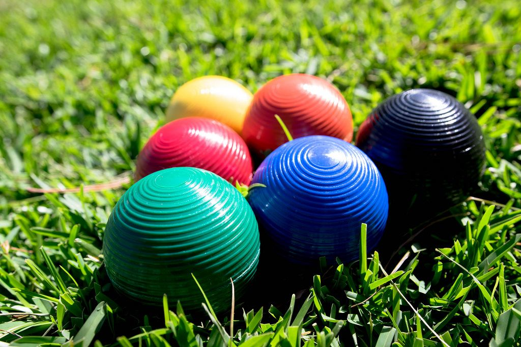
\includegraphics[width=80pt,height=60pt]{C6M04 - DT - Q1i.png}};
\draw (374.5,109.5) node  {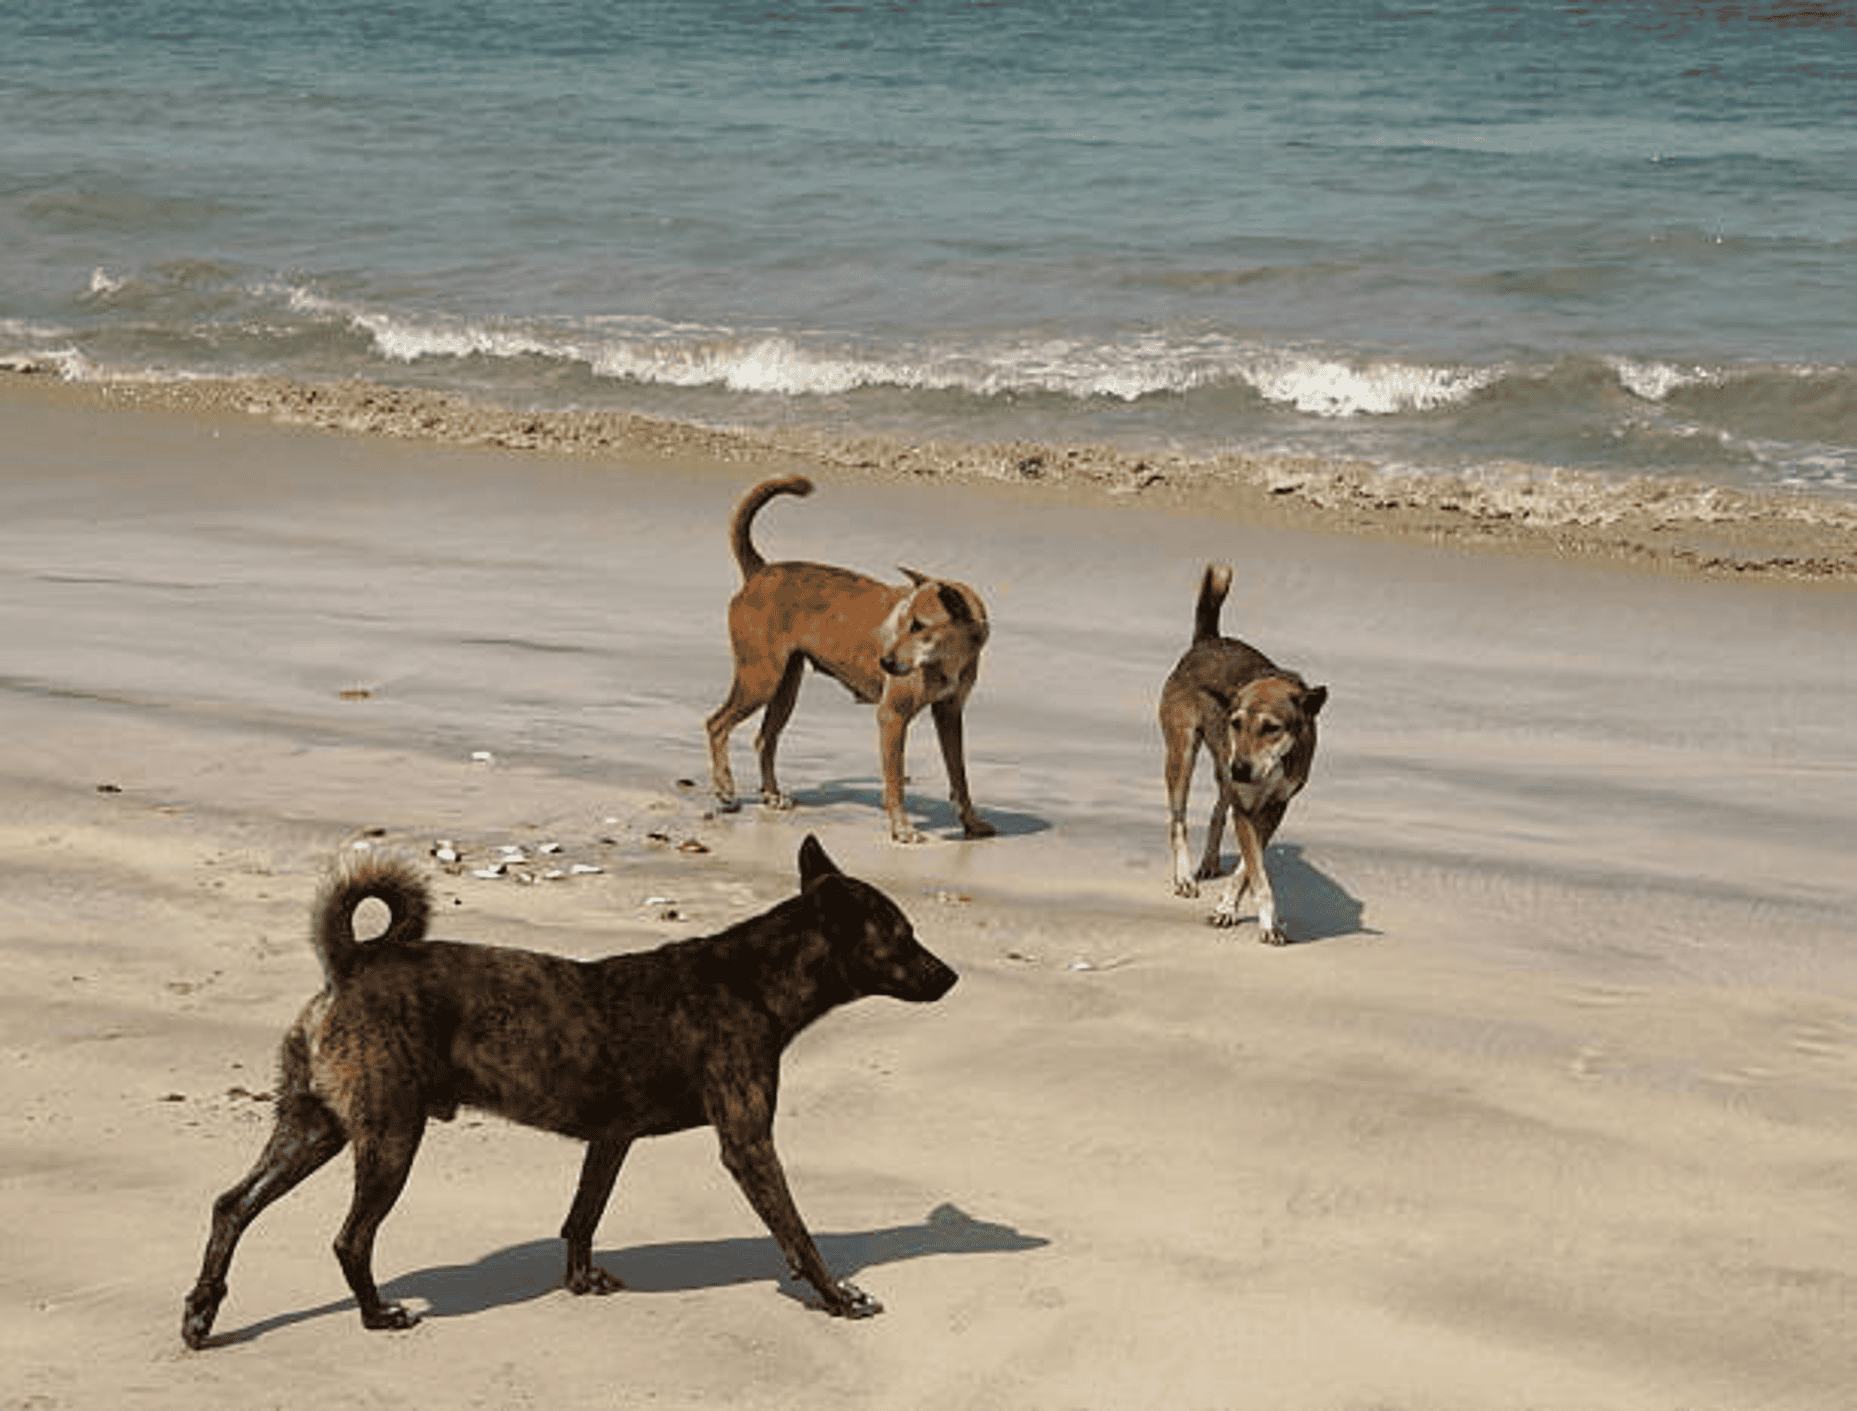
\includegraphics[width=80pt,height=60pt]{C6M04 - DT - Q1ii.png}};
\draw (90,155) node [anchor=north west][inner sep=0.75pt]   [align=left] {Number of balls = \rule{40pt}{0.5pt}};
\draw (295,155) node [anchor=north west][inner sep=0.75pt]   [align=left] {Number of dogs = \rule{40pt}{0.5pt}};
\end{tikzpicture}  
},
optionA={Balls},
optionB={Dogs},
optionC={Both balls and dogs},
optionD={None of these},
questionTag={C6M04 - DT - Q1}, 
leftmini={0.5},
rightmini={0.35},
correctoption={B},
}

\smallskip\centering
            \renewcommand{\arraystretch}{1.25}
            \begin{tabular}{|M{2cm}|M{1cm}|M{1cm}|M{1cm}|M{1cm}|M{1cm}|}
            \hline
Option & A (\ding{55}) & \cellcolor{cellgreen} B (\ding{51}) & C (\ding{55}) & D (\ding{55}) & E\\  
\hline
5 A & \highno{12\%} & \highno{65\%} & \highno{6\%} & \highno{6\%} & \highno{12\%} \\            \hline
\end{tabular}

\end{minipage}

\bigskip\answerkeychaptername{1 - Number System*}


\begin{minipage}{\linewidth}\mcqtextbottomOneFour{
questionnumber={4}, 
questionTag={C5M01 – DT – Q6},  
questiontext={Express the following in numbers.\\
\hspace{2cm}Four thousand nine hundred and two. },
optionA={492},
optionB={49002},
optionC={4092},
optionD={4902},
correctoption={D},
}

\smallskip\centering
            \renewcommand{\arraystretch}{1.25}
            \begin{tabular}{|M{2cm}|M{1cm}|M{1cm}|M{1cm}|M{1cm}|M{1cm}|}
            \hline
Option & A (\ding{55}) & B (\ding{55}) & C (\ding{55}) & \cellcolor{cellgreen} D (\ding{51}) & E\\  
\hline
5 A & \highno{18\%} & \highno{6\%} & \highno{6\%} & \highno{71\%} & \highno{0\%} \\            \hline
\end{tabular}

\end{minipage}

\bigskip


\begin{minipage}{\linewidth}\mcqtextbottomOneFour{
questionnumber={12}, 
questionTag={C5M01 – DT – Q7},  
questiontext={Arrange the following numbers in descending order.\\ \medskip
\hspace{4cm}367, 376, 389, 498 },
optionA={367, 376, 389, 498},
optionB={498, 389, 376, 367},
optionC={389, 498, 367, 376},
optionD={376, 399, 389, 367},
correctoption={B},
}

\smallskip\centering
            \renewcommand{\arraystretch}{1.25}
            \begin{tabular}{|M{2cm}|M{1cm}|M{1cm}|M{1cm}|M{1cm}|M{1cm}|}
            \hline
Option & A (\ding{55}) & \cellcolor{cellgreen} B (\ding{51}) & C (\ding{55}) & D (\ding{55}) & E\\  
\hline
5 A & \highno{6\%} & \highgreen{88\%} & \highno{6\%} & \highno{0\%} & \highno{0\%} \\            \hline
\end{tabular}

\end{minipage}

\bigskip


\begin{minipage}{\linewidth}\mcqtextbottomFourOne{
questionnumber={15}, 
questionTag={C5M01 – DT – Q10},  
questiontext={Write the number 79865 in words.},
optionA={Seven lakh eight hundred and sixty five},
optionB={Seventy nine eight hundred and sixty five},
optionC={Seven thousand eight hundred and sixty five},
optionD={Seventy nine thousand eight hundred and sixty five},
correctoption={D},
}

\smallskip\centering
            \renewcommand{\arraystretch}{1.25}
            \begin{tabular}{|M{2cm}|M{1cm}|M{1cm}|M{1cm}|M{1cm}|M{1cm}|}
            \hline
Option & A (\ding{55}) & B (\ding{55}) & C (\ding{55}) & \cellcolor{cellgreen} D (\ding{51}) & E\\  
\hline
5 A & \highno{0\%} & \highno{0\%} & \highno{0\%} & \highgreen{100\%} & \highno{0\%} \\            \hline
\end{tabular}

\end{minipage}

\bigskip


\begin{minipage}{\linewidth}\mcqtextbottomOneFour{
questionnumber={18}, 
questionTag={C5M01 – DT – Q8},  
questiontext={Solve the following and find which gives the greatest quotient.\\ \medskip
\hspace{4cm} i. 25$\divisionsymbol$5 \hspace{1cm} ii. 224$\divisionsymbol$2 \hspace{1cm}
iii. 66$\divisionsymbol$11},
optionA={i},
optionB={ii},
optionC={iii},
optionD={All are equal},
correctoption={B},
}

\smallskip\centering
            \renewcommand{\arraystretch}{1.25}
            \begin{tabular}{|M{2cm}|M{1cm}|M{1cm}|M{1cm}|M{1cm}|M{1cm}|}
            \hline
Option & A (\ding{55}) & \cellcolor{cellgreen} B (\ding{51}) & C (\ding{55}) & D (\ding{55}) & E\\  
\hline
5 A & \highno{6\%} & \highgreen{94\%} & \highno{0\%} & \highno{0\%} & \highno{0\%} \\            \hline
\end{tabular}

\end{minipage}

\bigskip


\begin{minipage}{\linewidth}\mcqtextbottomOneFour{
questionnumber={20}, 
questionTag={C5M01 – DT – Q1},  
questiontext={Find the sum. \qquad	234 + 908 = \rule{80pt}{0.5pt} },
optionA={1132},
optionB={1142},
optionC={1144},
optionD={11412},
correctoption={B},
}

\smallskip\centering
            \renewcommand{\arraystretch}{1.25}
            \begin{tabular}{|M{2cm}|M{1cm}|M{1cm}|M{1cm}|M{1cm}|M{1cm}|}
            \hline
Option & A (\ding{55}) & \cellcolor{cellgreen} B (\ding{51}) & C (\ding{55}) & D (\ding{55}) & E\\  
\hline
5 A & \highno{0\%} & \highgreen{94\%} & \highno{6\%} & \highno{0\%} & \highno{0\%} \\            \hline
\end{tabular}

\end{minipage}

\bigskip


\begin{minipage}{\linewidth}\mcqtextbottomOneFour{
questionnumber={26}, 
questionTag={C5M01 – DT – Q9},  
questiontext={Find the sum.\quad 524 + 98 = \rule{80pt}{0.5pt}},
optionA={612},
optionB={622},
optionC={1504},
optionD={51112},
correctoption={B},
}

\smallskip\centering
            \renewcommand{\arraystretch}{1.25}
            \begin{tabular}{|M{2cm}|M{1cm}|M{1cm}|M{1cm}|M{1cm}|M{1cm}|}
            \hline
Option & A (\ding{55}) & \cellcolor{cellgreen} B (\ding{51}) & C (\ding{55}) & D (\ding{55}) & E\\  
\hline
5 A & \highno{0\%} & \highgreen{94\%} & \highno{6\%} & \highno{0\%} & \highno{0\%} \\            \hline
\end{tabular}

\end{minipage}

\bigskip


\begin{minipage}{\linewidth}\mcqtextbottomOneFour{
questionnumber={27}, 
questionTag={C5M01 – DT – Q3},  
questiontext={Multiply.	\\ \medskip
\qquad i. 900 $\times$ 90 = \rule{80pt}{0.5pt} \qquad ii.  8 $\times$ 98 = \rule{80pt}{0.5pt} },
optionA={i. 8100, ii. 784},
optionB={i. 81000, ii.  724},
optionC={i. 81000, ii.  784},
optionD={i. 8100, ii. 724},
correctoption={C},
}

\smallskip\centering
            \renewcommand{\arraystretch}{1.25}
            \begin{tabular}{|M{2cm}|M{1cm}|M{1cm}|M{1cm}|M{1cm}|M{1cm}|}
            \hline
Option & A (\ding{55}) & B (\ding{55}) & \cellcolor{cellgreen} C (\ding{51}) & D (\ding{55}) & E\\  
\hline
5 A & \highno{12\%} & \highno{6\%} & \highgreen{76\%} & \highno{6\%} & \highno{0\%} \\            \hline
\end{tabular}

\end{minipage}

\bigskip


\begin{minipage}{\linewidth}\mcqtextbottomOneFour{
questionnumber={30}, 
questionTag={C5M01 – DT – Q5},  
questiontext={The place value of 5 in the number 05027 is \rule{80pt}{0.5pt} },
optionA={Hundreds},
optionB={Thousands},
optionC={Ones},
optionD={Tens},
correctoption={B},
}

\smallskip\centering
            \renewcommand{\arraystretch}{1.25}
            \begin{tabular}{|M{2cm}|M{1cm}|M{1cm}|M{1cm}|M{1cm}|M{1cm}|}
            \hline
Option & A (\ding{55}) & \cellcolor{cellgreen} B (\ding{51}) & C (\ding{55}) & D (\ding{55}) & E\\  
\hline
5 A & \highno{0\%} & \highgreen{94\%} & \highno{6\%} & \highno{0\%} & \highno{0\%} \\            \hline
\end{tabular}

\end{minipage}

\bigskip\answerkeychaptername{2 - Factor and Multiples*}


\begin{minipage}{\linewidth}\mcqtextbottomOneFour{
questionnumber={7}, 
questionTag={C5M02 – DT – Q3},  
questiontext={Identify the prime numbers.},
optionA={1},
optionB={0},
optionC={5},
optionD={10},
correctoption={C},
}

\smallskip\centering
            \renewcommand{\arraystretch}{1.25}
            \begin{tabular}{|M{2cm}|M{1cm}|M{1cm}|M{1cm}|M{1cm}|M{1cm}|}
            \hline
Option & A (\ding{55}) & B (\ding{55}) & \cellcolor{cellgreen} C (\ding{51}) & D (\ding{55}) & E\\  
\hline
5 A & \highno{6\%} & \highno{12\%} & \highno{71\%} & \highno{12\%} & \highno{0\%} \\            \hline
\end{tabular}

\end{minipage}

\bigskip


\begin{minipage}{\linewidth}\mcqtextbottomOneFour{
questionnumber={17}, 
questionTag={C5M02 – DT – Q2},  
questiontext={Find all the factors of 16. },
optionA={1, 2, 4},
optionB={1, 2, 4, 8},
optionC={1, 2, 4, 8, 16, 32},
optionD={1, 2, 4, 8, 16},
correctoption={D},
}

\smallskip\centering
            \renewcommand{\arraystretch}{1.25}
            \begin{tabular}{|M{2cm}|M{1cm}|M{1cm}|M{1cm}|M{1cm}|M{1cm}|}
            \hline
Option & A (\ding{55}) & B (\ding{55}) & C (\ding{55}) & \cellcolor{cellgreen} D (\ding{51}) & E\\  
\hline
5 A & \highno{0\%} & \highno{24\%} & \highno{6\%} & \highno{65\%} & \highno{6\%} \\            \hline
\end{tabular}

\end{minipage}

\bigskip


\begin{minipage}{\linewidth}\mcqtextbottomOneFour{
questionnumber={31}, 
questionTag={C5M02 – DT – Q1},  
questiontext={List the first four common multiples of 5 and 10. },
optionA={5, 10},
optionB={5, 10, 15, 20},
optionC={10, 20, 30, 40},
optionD={5, 15, 25, 35},
correctoption={C},
}

\smallskip\centering
            \renewcommand{\arraystretch}{1.25}
            \begin{tabular}{|M{2cm}|M{1cm}|M{1cm}|M{1cm}|M{1cm}|M{1cm}|}
            \hline
Option & A (\ding{55}) & B (\ding{55}) & \cellcolor{cellgreen} C (\ding{51}) & D (\ding{55}) & E\\  
\hline
5 A & \highno{35\%} & \highno{41\%} & \highred{18\%} & \highno{0\%} & \highno{6\%} \\            \hline
\end{tabular}

\end{minipage}

\bigskip


\begin{minipage}{\linewidth}\mcqtextbottomOneFour{
questionnumber={32}, 
questionTag={C5M02 – DT – Q4},  
questiontext={Find the multiples of 6.},
optionA={18, 24, 30, 36, 42},
optionB={24, 30, 36, 42, 49},
optionC={6, 8, 12, 18, 24},
optionD={6, 12, 16, 60, 66},
correctoption={A},
}

\smallskip\centering
            \renewcommand{\arraystretch}{1.25}
            \begin{tabular}{|M{2cm}|M{1cm}|M{1cm}|M{1cm}|M{1cm}|M{1cm}|}
            \hline
Option & \cellcolor{cellgreen} A (\ding{51}) & B (\ding{55}) & C (\ding{55}) & D (\ding{55}) & E\\  
\hline
5 A & \highno{65\%} & \highno{6\%} & \highno{6\%} & \highno{6\%} & \highno{18\%} \\            \hline
\end{tabular}

\end{minipage}

\bigskip\answerkeychaptername{3 - Fractions*}


\begin{minipage}{\linewidth}\mcqtextbottomOneFour{
questionnumber={6}, 
questionTag={C5M03 – DT – Q3},  
questiontext={Find the fraction of shaded portions.\\
\medskip
\tikzset{every picture/.style={line width=0.75pt}}
\hspace{4cm}
\begin{tikzpicture}[x=0.75pt,y=0.75pt,yscale=-1,xscale=1]
\draw  [fill={rgb, 255:red, 155; green, 155; blue, 155 }  ,fill opacity=1 ] (60.5,50.5) -- (120.5,50.5) -- (120.5,79) -- (60.5,79) -- cycle ;
\draw  [fill={rgb, 255:red, 155; green, 155; blue, 155 }  ,fill opacity=1 ] (121,50.5) -- (181,50.5) -- (181,79) -- (121,79) -- cycle ;
\draw   (180.5,50.5) -- (240.5,50.5) -- (240.5,79) -- (180.5,79) -- cycle ;
\draw   (240.5,50.5) -- (300.5,50.5) -- (300.5,79) -- (240.5,79) -- cycle ;
\draw   (300.5,50.5) -- (360.5,50.5) -- (360.5,79) -- (300.5,79) -- cycle ;
\draw  [fill={rgb, 255:red, 155; green, 155; blue, 155 }  ,fill opacity=1 ] (60.5,80) -- (120.5,80) -- (120.5,108.5) -- (60.5,108.5) -- cycle ;
\draw  [fill={rgb, 255:red, 155; green, 155; blue, 155 }  ,fill opacity=1 ] (121,80) -- (181,80) -- (181,108.5) -- (121,108.5) -- cycle ;
\draw   (180.5,80) -- (240.5,80) -- (240.5,108.5) -- (180.5,108.5) -- cycle ;
\draw   (240.5,80) -- (300.5,80) -- (300.5,108.5) -- (240.5,108.5) -- cycle ;
\draw   (300.5,80) -- (360.5,80) -- (360.5,108.5) -- (300.5,108.5) -- cycle ;
\end{tikzpicture} 
},
optionA={$\frac{6}{10}$},
optionB={$\frac{2}{3}$},
optionC={$\frac{4}{6}$},
optionD={$\frac{4}{10}$},
correctoption={D},
}

\smallskip\centering
            \renewcommand{\arraystretch}{1.25}
            \begin{tabular}{|M{2cm}|M{1cm}|M{1cm}|M{1cm}|M{1cm}|M{1cm}|}
            \hline
Option & A (\ding{55}) & B (\ding{55}) & C (\ding{55}) & \cellcolor{cellgreen} D (\ding{51}) & E\\  
\hline
5 A & \highno{0\%} & \highno{0\%} & \highno{24\%} & \highno{71\%} & \highno{6\%} \\            \hline
\end{tabular}

\end{minipage}

\bigskip


\begin{minipage}{\linewidth}\mcqtextbottomOneFour{
questionnumber={13}, 
questionTag={C5M03 – DT – Q1},  
questiontext={Find the square that has one fourth shaded portion. },
optionA={
\tikzset{every picture/.style={line width=0.75pt}} 
\begin{tikzpicture}[x=0.75pt,y=0.75pt,yscale=-1,xscale=1]
\draw  [fill={rgb, 255:red, 155; green, 155; blue, 155 }  ,fill opacity=1 ] (115,139.94) -- (141.28,139.94) -- (141.28,166.22) -- (115,166.22) -- cycle ;
\draw   (141.28,139.94) -- (167.57,139.94) -- (167.57,166.22) -- (141.28,166.22) -- cycle ;
\draw   (115,166.22) -- (141.28,166.22) -- (141.28,192.51) -- (115,192.51) -- cycle ;
\draw   (141.28,166.22) -- (167.57,166.22) -- (167.57,192.51) -- (141.28,192.51) -- cycle ;
\end{tikzpicture} },
optionB={
\tikzset{every picture/.style={line width=0.75pt}}
\begin{tikzpicture}[x=0.75pt,y=0.75pt,yscale=-1,xscale=1]
\draw  [fill={rgb, 255:red, 155; green, 155; blue, 155 }  ,fill opacity=1 ] (178.96,139.94) -- (205.24,139.94) -- (205.24,166.22) -- (178.96,166.22) -- cycle ;
\draw  [fill={rgb, 255:red, 155; green, 155; blue, 155 }  ,fill opacity=1 ] (205.24,139.94) -- (231.52,139.94) -- (231.52,166.22) -- (205.24,166.22) -- cycle ; 
\draw   (178.96,166.22) -- (205.24,166.22) -- (205.24,192.51) -- (178.96,192.51) -- cycle ;
\draw   (205.24,166.22) -- (231.52,166.22) -- (231.52,192.51) -- (205.24,192.51) -- cycle ;
\end{tikzpicture}},
optionC={
\tikzset{every picture/.style={line width=0.75pt}}
\begin{tikzpicture}[x=0.75pt,y=0.75pt,yscale=-1,xscale=1] 
\draw  [fill={rgb, 255:red, 155; green, 155; blue, 155 }  ,fill opacity=1 ] (242.91,139.94) -- (269.2,139.94) -- (269.2,166.22) -- (242.91,166.22) -- cycle ;
\draw  [fill={rgb, 255:red, 155; green, 155; blue, 155 }  ,fill opacity=1 ] (269.2,139.94) -- (295.48,139.94) -- (295.48,166.22) -- (269.2,166.22) -- cycle ;
\draw  [fill={rgb, 255:red, 155; green, 155; blue, 155 }  ,fill opacity=1 ] (242.91,166.22) -- (269.2,166.22) -- (269.2,192.51) -- (242.91,192.51) -- cycle ;
\draw   (269.2,166.22) -- (295.48,166.22) -- (295.48,192.51) -- (269.2,192.51) -- cycle ;
\end{tikzpicture}},
optionD={
\tikzset{every picture/.style={line width=0.75pt}} 
\begin{tikzpicture}[x=0.75pt,y=0.75pt,yscale=-1,xscale=1]
\draw  [fill={rgb, 255:red, 155; green, 155; blue, 155 }  ,fill opacity=1 ] (306.43,139.5) -- (332.72,139.5) -- (332.72,165.78) -- (306.43,165.78) -- cycle ;
\draw  [fill={rgb, 255:red, 155; green, 155; blue, 155 }  ,fill opacity=1 ] (332.72,139.5) -- (359,139.5) -- (359,165.78) -- (332.72,165.78) -- cycle ; 
\draw  [fill={rgb, 255:red, 155; green, 155; blue, 155 }  ,fill opacity=1 ] (306.43,165.78) -- (332.72,165.78) -- (332.72,192.07) -- (306.43,192.07) -- cycle ; 
\draw  [fill={rgb, 255:red, 155; green, 155; blue, 155 }  ,fill opacity=1 ] (332.72,165.78) -- (359,165.78) -- (359,192.07) -- (332.72,192.07) -- cycle ;
\end{tikzpicture}},
correctoption={A},
}

\smallskip\centering
            \renewcommand{\arraystretch}{1.25}
            \begin{tabular}{|M{2cm}|M{1cm}|M{1cm}|M{1cm}|M{1cm}|M{1cm}|}
            \hline
Option & \cellcolor{cellgreen} A (\ding{51}) & B (\ding{55}) & C (\ding{55}) & D (\ding{55}) & E\\  
\hline
5 A & \highno{47\%} & \highno{0\%} & \highno{6\%} & \highno{35\%} & \highno{12\%} \\            \hline
\end{tabular}

\end{minipage}

\bigskip


\begin{minipage}{\linewidth}\mcqtextbottomOneFour{
questionnumber={37}, 
questionTag={C5M03 – DT – Q2},  
questiontext={What is the half of 50? },
optionA={5},
optionB={50},
optionC={25},
optionD={100},
correctoption={C},
}

\smallskip\centering
            \renewcommand{\arraystretch}{1.25}
            \begin{tabular}{|M{2cm}|M{1cm}|M{1cm}|M{1cm}|M{1cm}|M{1cm}|}
            \hline
Option & A (\ding{55}) & B (\ding{55}) & \cellcolor{cellgreen} C (\ding{51}) & D (\ding{55}) & E\\  
\hline
5 A & \highno{6\%} & \highno{6\%} & \highgreen{82\%} & \highno{6\%} & \highno{0\%} \\            \hline
\end{tabular}

\end{minipage}

\bigskip\answerkeychaptername{4 - Decimals and their Conversion*}


\begin{minipage}{\linewidth}\mcqtextbottomOneFour{
questionnumber={9}, 
questionTag={C5M04 – DT – Q3},  
questiontext={ Express 25 paise in rupees.},
optionA={Rs. 0.25},
optionB={Rs. 2.5},
optionC={Rs. 2500},
optionD={Rs. 25},
correctoption={A},
}

\smallskip\centering
            \renewcommand{\arraystretch}{1.25}
            \begin{tabular}{|M{2cm}|M{1cm}|M{1cm}|M{1cm}|M{1cm}|M{1cm}|}
            \hline
Option & \cellcolor{cellgreen} A (\ding{51}) & B (\ding{55}) & C (\ding{55}) & D (\ding{55}) & E\\  
\hline
5 A & \highno{41\%} & \highno{24\%} & \highno{12\%} & \highno{12\%} & \highno{12\%} \\            \hline
\end{tabular}

\end{minipage}

\bigskip


\begin{minipage}{\linewidth}\mcqtextbottomOneFour{
questionnumber={14}, 
questionTag={C5M04 – DT – Q4},  
questiontext={10 cm = \rule{80pt}{0.5pt} mm},
optionA={10 mm},
optionB={100 mm},
optionC={1 mm},
optionD={0.01 mm},
correctoption={B},
}

\smallskip\centering
            \renewcommand{\arraystretch}{1.25}
            \begin{tabular}{|M{2cm}|M{1cm}|M{1cm}|M{1cm}|M{1cm}|M{1cm}|}
            \hline
Option & A (\ding{55}) & \cellcolor{cellgreen} B (\ding{51}) & C (\ding{55}) & D (\ding{55}) & E\\  
\hline
5 A & \highno{6\%} & \highno{59\%} & \highno{29\%} & \highno{0\%} & \highno{6\%} \\            \hline
\end{tabular}

\end{minipage}

\bigskip


\begin{minipage}{\linewidth}\mcqtextbottomOneFour{
questionnumber={19}, 
questionTag={C5M04 – DT – Q2},  
questiontext={Ram bought 23.5 kg of tomatoes. Help him to represent 23.5 kg in grams. },
optionA={23500 g},
optionB={2350 g},
optionC={23.5000 g},
optionD={235 g},
correctoption={A},
}

\smallskip\centering
            \renewcommand{\arraystretch}{1.25}
            \begin{tabular}{|M{2cm}|M{1cm}|M{1cm}|M{1cm}|M{1cm}|M{1cm}|}
            \hline
Option & \cellcolor{cellgreen} A (\ding{51}) & B (\ding{55}) & C (\ding{55}) & D (\ding{55}) & E\\  
\hline
5 A & \highred{12\%} & \highno{24\%} & \highno{35\%} & \highno{24\%} & \highno{6\%} \\            \hline
\end{tabular}

\end{minipage}

\bigskip


\begin{minipage}{\linewidth}\mcqtextbottomOneFour{
questionnumber={23}, 
questionTag={C5M04 – DT – Q7},  
questiontext={Ramu has 5000 ml of water. How many 1-liter bottles will he need to hold it?},
optionA={5},
optionB={6},
optionC={55},
optionD={100},
correctoption={A},
}

\smallskip\centering
            \renewcommand{\arraystretch}{1.25}
            \begin{tabular}{|M{2cm}|M{1cm}|M{1cm}|M{1cm}|M{1cm}|M{1cm}|}
            \hline
Option & \cellcolor{cellgreen} A (\ding{51}) & B (\ding{55}) & C (\ding{55}) & D (\ding{55}) & E\\  
\hline
5 A & \highno{41\%} & \highno{12\%} & \highno{24\%} & \highno{18\%} & \highno{6\%} \\            \hline
\end{tabular}

\end{minipage}

\bigskip


\begin{minipage}{\linewidth}\mcqtextbottomOneFour{
questionnumber={33}, 
questionTag={C5M04 – DT – Q1},  
questiontext={The representation of the fraction {\large{$\frac{1}{100}$}} in decimal form is \rule{80pt}{0.5pt}},
optionA={0.1},
optionB={0.01},
optionC={0.001},
optionD={1},
correctoption={B},
}

\smallskip\centering
            \renewcommand{\arraystretch}{1.25}
            \begin{tabular}{|M{2cm}|M{1cm}|M{1cm}|M{1cm}|M{1cm}|M{1cm}|}
            \hline
Option & A (\ding{55}) & \cellcolor{cellgreen} B (\ding{51}) & C (\ding{55}) & D (\ding{55}) & E\\  
\hline
5 A & \highno{0\%} & \highgreen{88\%} & \highno{6\%} & \highno{6\%} & \highno{0\%} \\            \hline
\end{tabular}

\end{minipage}

\bigskip


\begin{minipage}{\linewidth}\mcqtextbottomOneFour{
questionnumber={38}, 
questionTag={C5M04 – DT – Q5},  
questiontext={Which unit is used to measure the quantity of water in a bucket?},
optionA={Kilometer},
optionB={Liter},
optionC={Meter},
optionD={Decigram},
correctoption={B},
}

\smallskip\centering
            \renewcommand{\arraystretch}{1.25}
            \begin{tabular}{|M{2cm}|M{1cm}|M{1cm}|M{1cm}|M{1cm}|M{1cm}|}
            \hline
Option & A (\ding{55}) & \cellcolor{cellgreen} B (\ding{51}) & C (\ding{55}) & D (\ding{55}) & E\\  
\hline
5 A & \highno{0\%} & \highgreen{88\%} & \highno{6\%} & \highno{0\%} & \highno{6\%} \\            \hline
\end{tabular}

\end{minipage}

\bigskip


\begin{minipage}{\linewidth}\mcqtextbottomOneFour{
questionnumber={39}, 
questionTag={C5M04 – DT – Q6},  
questiontext={Find the time duration between 9:15 AM and 11:45 AM.},
optionA={2 hours},
optionB={1.5 hours},
optionC={2.25 hours},
optionD={2.5 hours},
correctoption={D},
}

\smallskip\centering
            \renewcommand{\arraystretch}{1.25}
            \begin{tabular}{|M{2cm}|M{1cm}|M{1cm}|M{1cm}|M{1cm}|M{1cm}|}
            \hline
Option & A (\ding{55}) & B (\ding{55}) & C (\ding{55}) & \cellcolor{cellgreen} D (\ding{51}) & E\\  
\hline
5 A & \highno{29\%} & \highno{12\%} & \highno{29\%} & \highred{12\%} & \highno{18\%} \\            \hline
\end{tabular}

\end{minipage}

\bigskip\answerkeychaptername{5 - Shapes and Angles*}


\begin{minipage}{\linewidth}\mcqimgleftFourOne{
questionnumber={21}, 
questionTag={C5M05 – DT – Q1}, 
questiontext={Identify the number of sides in the given figure.},
imgtabletikz = { 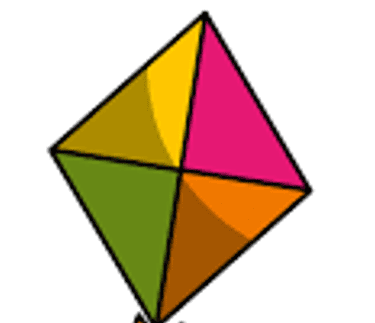
\includegraphics[height= 2.5cm, width= 3.5 cm]{C5M05 – DT – Q1.png}},
optionA={No sides},
optionB={Six sides},
optionC={Four sides},
optionD={Three sides},
correctoption={C},
leftmini={0.5},
rightmini={0.4},
}

\smallskip\centering
            \renewcommand{\arraystretch}{1.25}
            \begin{tabular}{|M{2cm}|M{1cm}|M{1cm}|M{1cm}|M{1cm}|M{1cm}|}
            \hline
Option & A (\ding{55}) & B (\ding{55}) & \cellcolor{cellgreen} C (\ding{51}) & D (\ding{55}) & E\\  
\hline
5 A & \highno{0\%} & \highno{0\%} & \highgreen{100\%} & \highno{0\%} & \highno{0\%} \\            \hline
\end{tabular}

\end{minipage}

\bigskip


\begin{minipage}{\linewidth}\mcqimgleftFourOne{
questionnumber={22}, 
questionTag={C5M05 – DT – Q3},  
questiontext={In the given figure, the angle formed is \rule{80pt}{0.5pt} the right angle. },
imgtabletikz = { 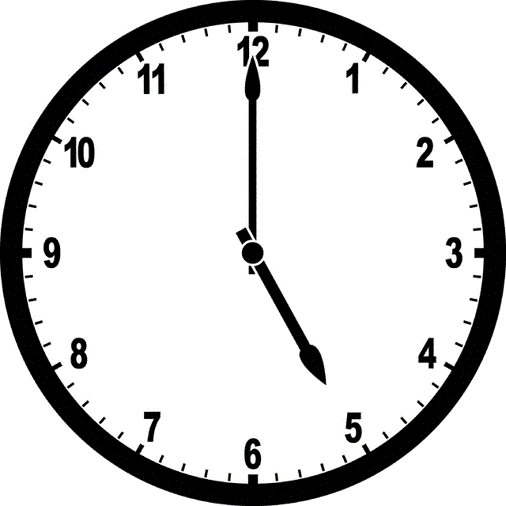
\includegraphics[height= 3cm, width= 3 cm]{C5M05 – DT – Q3.png}},
optionA={Equal to},
optionB={Greater than},
optionC={Lesser than},
optionD={Not equal to},
correctoption={B},
leftmini={0.6},
rightmini={0.3},
}

\smallskip\centering
            \renewcommand{\arraystretch}{1.25}
            \begin{tabular}{|M{2cm}|M{1cm}|M{1cm}|M{1cm}|M{1cm}|M{1cm}|}
            \hline
Option & A (\ding{55}) & \cellcolor{cellgreen} B (\ding{51}) & C (\ding{55}) & D (\ding{55}) & E\\  
\hline
5 A & \highno{12\%} & \highred{35\%} & \highno{29\%} & \highno{18\%} & \highno{6\%} \\            \hline
\end{tabular}

\end{minipage}

\bigskip


\begin{minipage}{\linewidth}\mcqimgleftFourOne{
questionnumber={29}, 
questionTag={C5M05 – DT – Q2},  
questiontext={Find the length of pencil. },
imgtabletikz = { 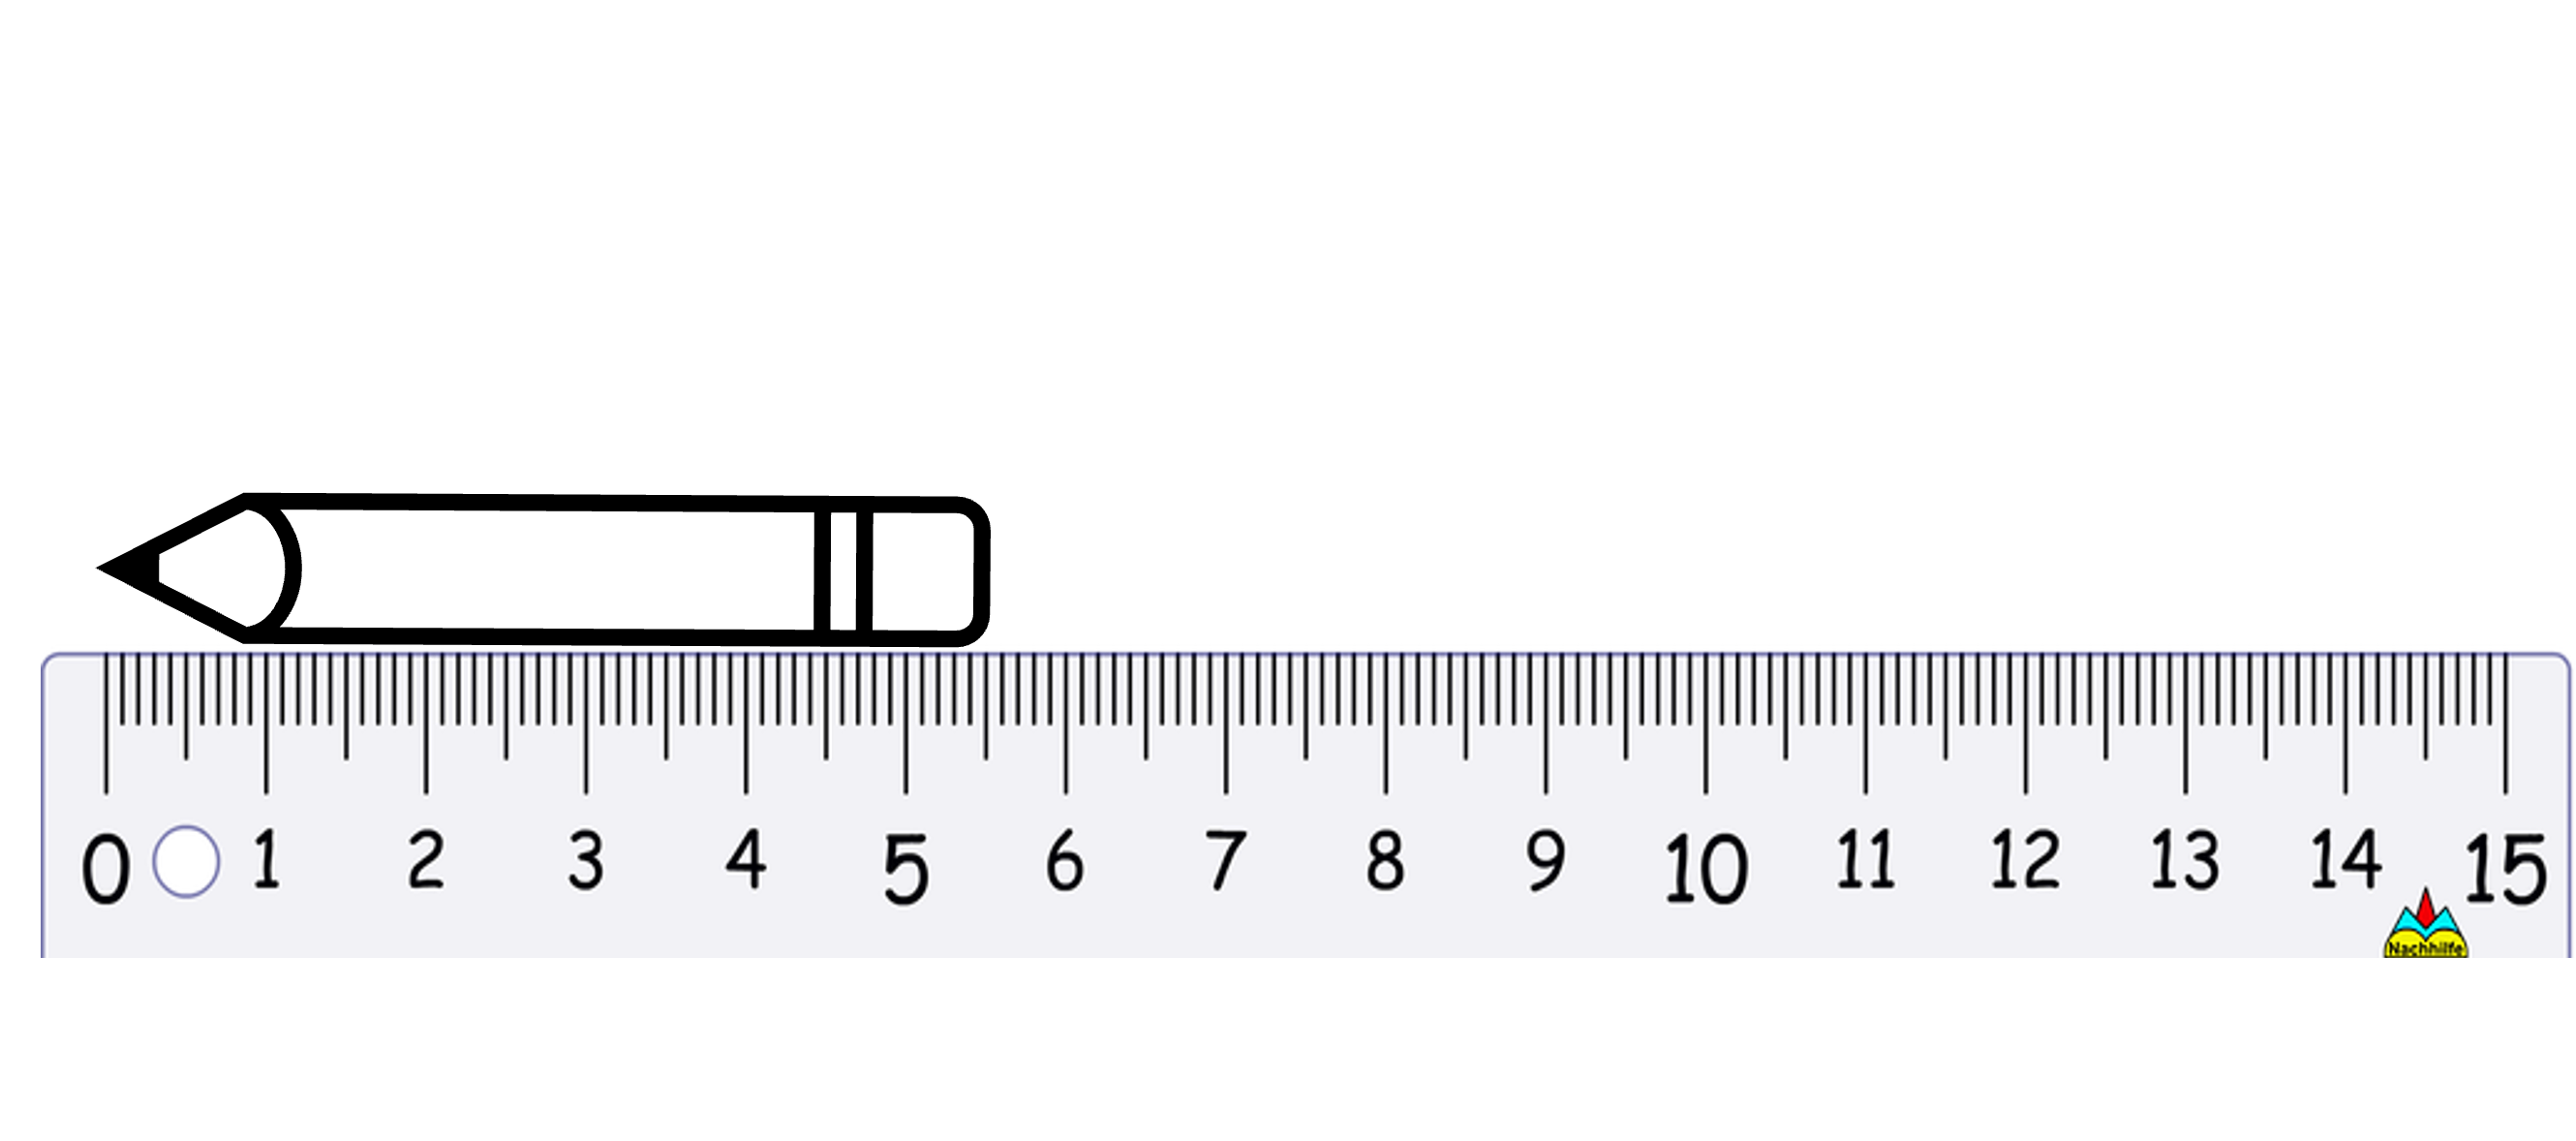
\includegraphics[height= 3cm, width= 10 cm]{C5M05 – DT – Q2.png}},
optionA={6.5 cm},
optionB={5.5 cm},
optionC={5 cm},
optionD={6 cm},
correctoption={B},
leftmini={0.6},
rightmini={0.3},
}

\smallskip\centering
            \renewcommand{\arraystretch}{1.25}
            \begin{tabular}{|M{2cm}|M{1cm}|M{1cm}|M{1cm}|M{1cm}|M{1cm}|}
            \hline
Option & A (\ding{55}) & \cellcolor{cellgreen} B (\ding{51}) & C (\ding{55}) & D (\ding{55}) & E\\  
\hline
5 A & \highno{6\%} & \highgreen{94\%} & \highno{0\%} & \highno{0\%} & \highno{0\%} \\            \hline
\end{tabular}

\end{minipage}

\bigskip\answerkeychaptername{6 - Visualization*}


\begin{minipage}{\linewidth}\mcqimgleftFourOne{
questionnumber={25}, 
questionTag={C5M06 – DT – Q2},  
questiontext={ Identify the shape of the following image.},
imgtabletikz = { 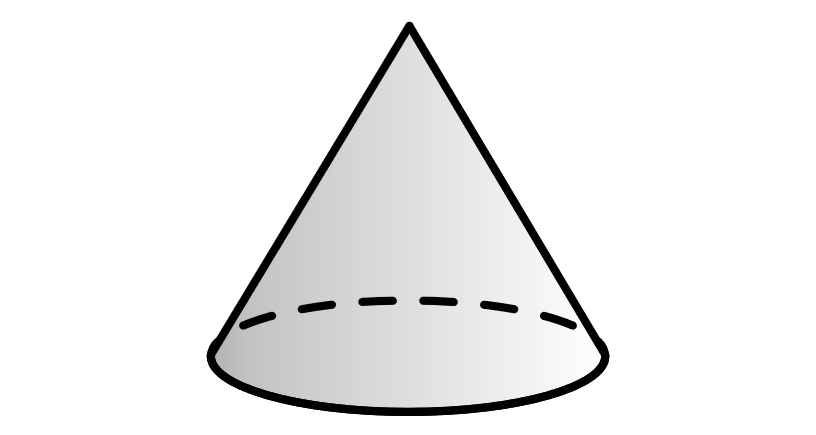
\includegraphics[height= 2.5 cm, width= 5 cm]{C5M06 – DT – Q2.png}},
optionA={Cube},
optionB={Cuboid},
optionC={Cone},
optionD={Cylinder},
correctoption={C},
leftmini={0.6},
rightmini={0.3},
}

\smallskip\centering
            \renewcommand{\arraystretch}{1.25}
            \begin{tabular}{|M{2cm}|M{1cm}|M{1cm}|M{1cm}|M{1cm}|M{1cm}|}
            \hline
Option & A (\ding{55}) & B (\ding{55}) & \cellcolor{cellgreen} C (\ding{51}) & D (\ding{55}) & E\\  
\hline
5 A & \highno{0\%} & \highno{12\%} & \highgreen{88\%} & \highno{0\%} & \highno{0\%} \\            \hline
\end{tabular}

\end{minipage}

\bigskip


\begin{minipage}{\linewidth}\mcqtextbottomOneFour{
questionnumber={28}, 
questionTag={C5M06 – DT – Q1},  
questiontext={Ajaykanth got a salary of Rs.10,000 in January month, Rs.12,000 in February month, Rs. 14,000 in March month and the pattern continued. How much he had earned in the month of June? },
optionA={Rs. 18,000},
optionB={Rs. 16,000},
optionC={Rs. 15,000},
optionD={Rs. 20,000},
correctoption={D},
}

\smallskip\centering
            \renewcommand{\arraystretch}{1.25}
            \begin{tabular}{|M{2cm}|M{1cm}|M{1cm}|M{1cm}|M{1cm}|M{1cm}|}
            \hline
Option & A (\ding{55}) & B (\ding{55}) & C (\ding{55}) & \cellcolor{cellgreen} D (\ding{51}) & E\\  
\hline
5 A & \highno{12\%} & \highno{53\%} & \highno{6\%} & \highred{24\%} & \highno{6\%} \\            \hline
\end{tabular}

\end{minipage}

\bigskip\answerkeychaptername{7 - Symmetry*}


\begin{minipage}{\linewidth}\mcqtextbottomOneFour{
questionnumber={3}, 
questionTag={C5M07 – DT – Q2},  
questiontext={Pick the shape which is not divided into two mirror halves by the dotted line.\\
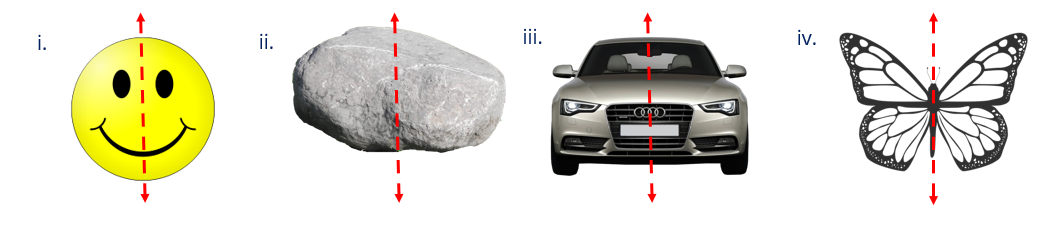
\includegraphics[height= 3.5cm, width= 16 cm]{C5M07 – DT – Q2.png}
},
optionA={i},
optionB={ii},
optionC={iii},
optionD={iv},
correctoption={B},
}

\smallskip\centering
            \renewcommand{\arraystretch}{1.25}
            \begin{tabular}{|M{2cm}|M{1cm}|M{1cm}|M{1cm}|M{1cm}|M{1cm}|}
            \hline
Option & A (\ding{55}) & \cellcolor{cellgreen} B (\ding{51}) & C (\ding{55}) & D (\ding{55}) & E\\  
\hline
5 A & \highno{6\%} & \highgreen{76\%} & \highno{12\%} & \highno{6\%} & \highno{0\%} \\            \hline
\end{tabular}

\end{minipage}

\bigskip\answerkeychaptername{8 - Mensuration*}


\begin{minipage}{\linewidth}\mcqtextbottomOneFour{
questionnumber={11}, 
questionTag={C5M08 – DT – Q2},  
questiontext={Find the perimeter of the rectangle if its length and breadth is 10 cm and 4 cm respectively. },
optionA={14 cm},
optionB={28 cm},
optionC={40 cm},
optionD={104 cm},
correctoption={B},
}

\smallskip\centering
            \renewcommand{\arraystretch}{1.25}
            \begin{tabular}{|M{2cm}|M{1cm}|M{1cm}|M{1cm}|M{1cm}|M{1cm}|}
            \hline
Option & A (\ding{55}) & \cellcolor{cellgreen} B (\ding{51}) & C (\ding{55}) & D (\ding{55}) & E\\  
\hline
5 A & \highno{18\%} & \highno{47\%} & \highno{29\%} & \highno{6\%} & \highno{0\%} \\            \hline
\end{tabular}

\end{minipage}

\bigskip


\begin{minipage}{\linewidth}\mcqimgleftFourOne{
questionnumber={24}, 
questionTag={C5M08 – DT – Q3},  
questiontext={Find the area of the rectangle. },
imgtabletikz = { 
\tikzset{every picture/.style={line width=0.75pt}} 
\begin{tikzpicture}[x=0.75pt,y=0.75pt,yscale=-1,xscale=1]
\draw  [fill={rgb, 255:red, 155; green, 155; blue, 155 }  ,fill opacity=0.48 ] (122,102) -- (294,102) -- (294,179) -- (122,179) -- cycle ;
\draw (186,80) node [anchor=north west][inner sep=0.75pt]   [align=left] {20 cm};
\draw (299,127) node [anchor=north west][inner sep=0.75pt]   [align=left] {8 cm};
\end{tikzpicture} },
optionA={12 sq. cm},
optionB={28 sq. cm},
optionC={56 sq. cm},
optionD={160 sq.cm},
correctoption={D},
leftmini={0.6},
rightmini={0.3},
}

\smallskip\centering
            \renewcommand{\arraystretch}{1.25}
            \begin{tabular}{|M{2cm}|M{1cm}|M{1cm}|M{1cm}|M{1cm}|M{1cm}|}
            \hline
Option & A (\ding{55}) & B (\ding{55}) & C (\ding{55}) & \cellcolor{cellgreen} D (\ding{51}) & E\\  
\hline
5 A & \highno{0\%} & \highno{24\%} & \highno{24\%} & \highno{53\%} & \highno{0\%} \\            \hline
\end{tabular}

\end{minipage}

\bigskip


\begin{minipage}{\linewidth}\mcqimgleftFourOne{
questionnumber={36}, 
questionTag={C5M08 – DT – Q1},  
questiontext={Find the area of the following shaded squares, if the side of one square is 1 cm. },
imgtabletikz = { 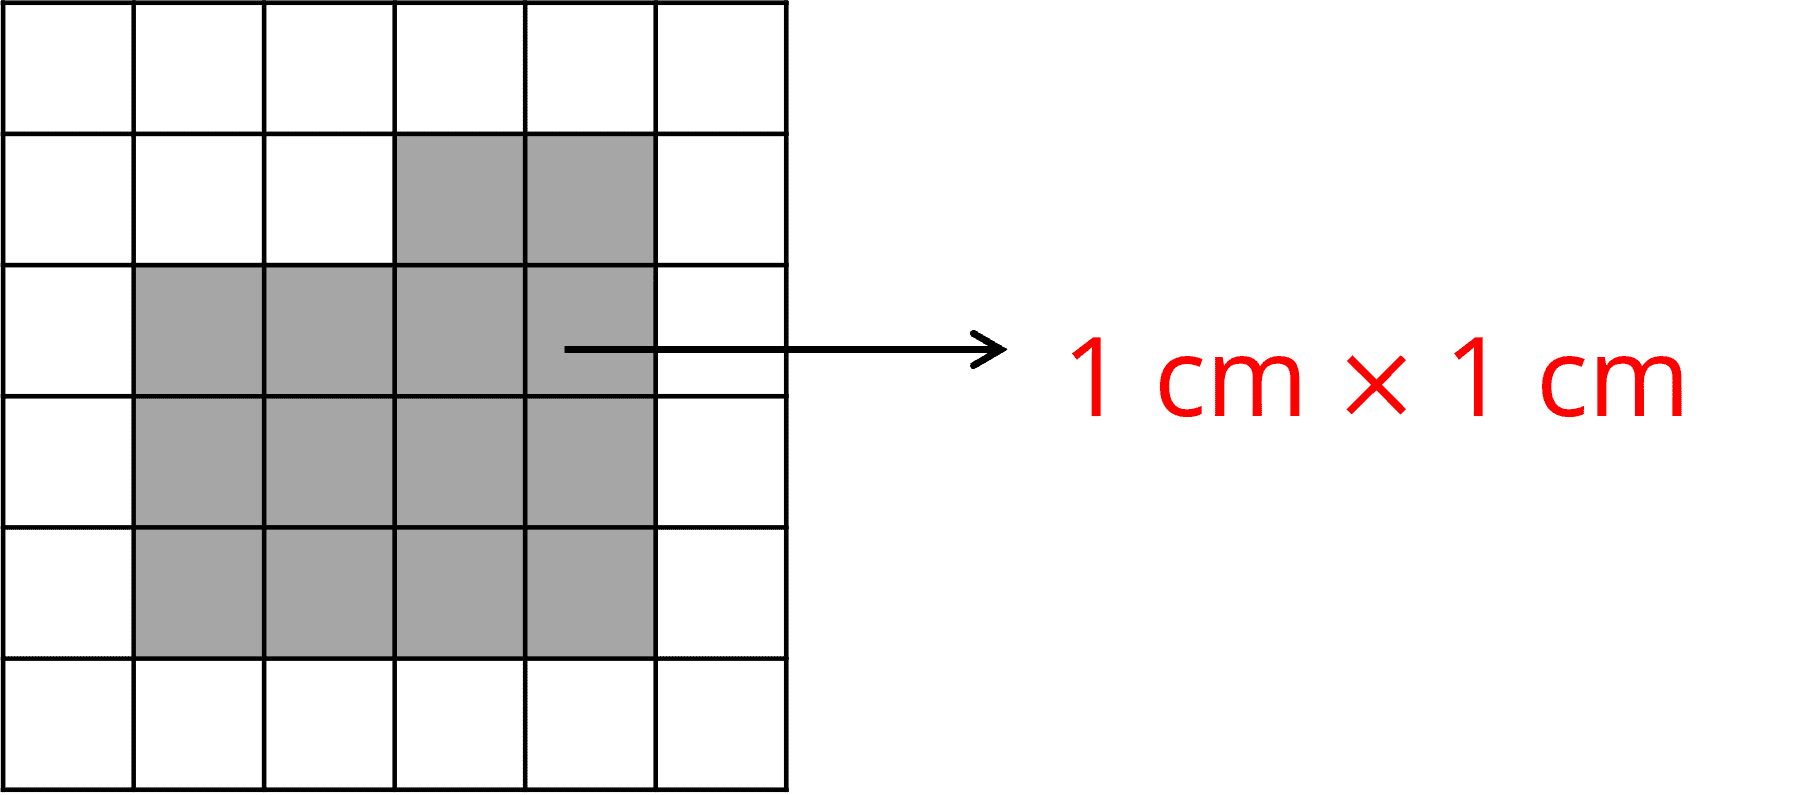
\includegraphics[height= 2.5cm, width= 6 cm]{C5M08 – DT – Q1.png}},
optionA={28 sq. cm},
optionB={56 sq. cm},
optionC={14 sq. cm},
optionD={7 sq. cm},
correctoption={C},
leftmini={0.6},
rightmini={0.3},
}

\smallskip\centering
            \renewcommand{\arraystretch}{1.25}
            \begin{tabular}{|M{2cm}|M{1cm}|M{1cm}|M{1cm}|M{1cm}|M{1cm}|}
            \hline
Option & A (\ding{55}) & B (\ding{55}) & \cellcolor{cellgreen} C (\ding{51}) & D (\ding{55}) & E\\  
\hline
5 A & \highno{0\%} & \highno{0\%} & \highgreen{94\%} & \highno{0\%} & \highno{6\%} \\            \hline
\end{tabular}

\end{minipage}

\bigskip\answerkeychaptername{9 - Charts*}


\begin{minipage}{\linewidth}\mcqimgleftFourOne{
questionnumber={16}, 
questionTag={C5M09 – DT – Q2},  
questiontext={Which genre is liked more? },
imgtabletikz = { 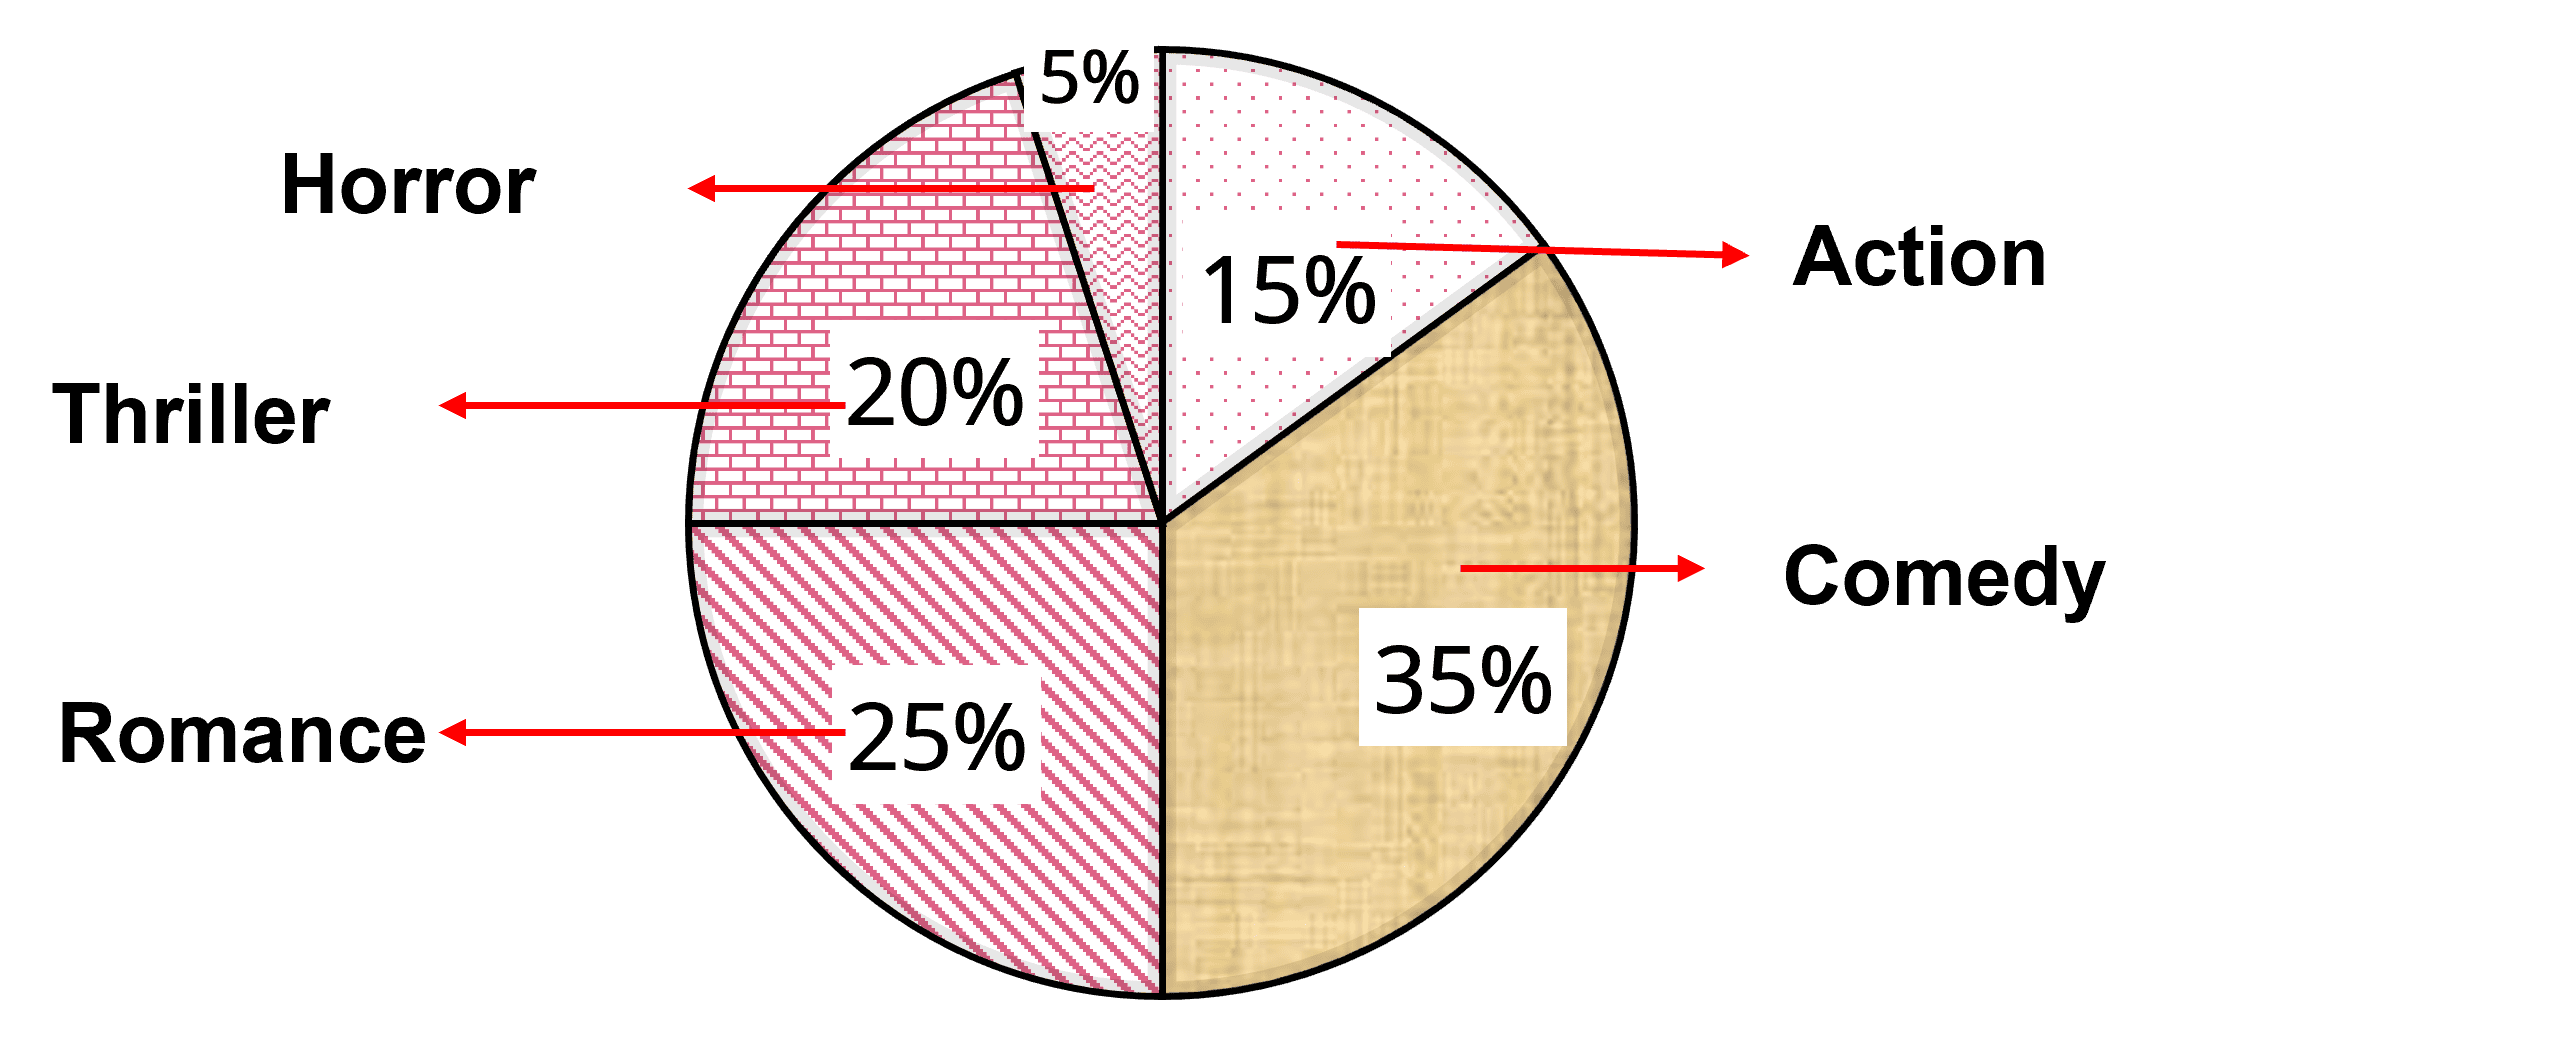
\includegraphics[height= 4cm, width= 10 cm]{C5M09 – DT – Q2.png}},
optionA={Comedy},
optionB={Horror},
optionC={Thriller},
optionD={Romance},
correctoption={A},
leftmini={0.6},
rightmini={0.3},
}

\smallskip\centering
            \renewcommand{\arraystretch}{1.25}
            \begin{tabular}{|M{2cm}|M{1cm}|M{1cm}|M{1cm}|M{1cm}|M{1cm}|}
            \hline
Option & \cellcolor{cellgreen} A (\ding{51}) & B (\ding{55}) & C (\ding{55}) & D (\ding{55}) & E\\  
\hline
5 A & \highgreen{100\%} & \highno{0\%} & \highno{0\%} & \highno{0\%} & \highno{0\%} \\            \hline
\end{tabular}

\end{minipage}

\bigskip


\begin{minipage}{\linewidth}\mcqtextbottomOneFour{
questionnumber={40}, 
questionTag={C5M09 – DT – Q1},  
questiontext={Find the number for the tally mark representation of \tikzset{every picture/.style={line width=0.75pt}} 
\begin{tikzpicture}[x=0.75pt,y=0.75pt,yscale=-1,xscale=1] 
\draw    (98.33,161.14) -- (98.33,183.39) ;
\draw    (110.28,161) -- (110.28,183.25) ;
\draw    (121.36,161.28) -- (121.36,183.53) ;
\draw    (133.31,161.42) -- (133.31,183.67) ;
\draw    (133.31,161.42) -- (98.33,183.39) ;
\draw    (145.26,161) -- (145.26,183.25) ;
\end{tikzpicture} },
optionA={8},
optionB={6},
optionC={7},
optionD={5},
correctoption={B},
}

\smallskip\centering
            \renewcommand{\arraystretch}{1.25}
            \begin{tabular}{|M{2cm}|M{1cm}|M{1cm}|M{1cm}|M{1cm}|M{1cm}|}
            \hline
Option & A (\ding{55}) & \cellcolor{cellgreen} B (\ding{51}) & C (\ding{55}) & D (\ding{55}) & E\\  
\hline
5 A & \highno{6\%} & \highno{71\%} & \highno{0\%} & \highno{24\%} & \highno{0\%} \\            \hline
\end{tabular}

\end{minipage}

\bigskip\answerkeychaptername{17 - Data Handling *}


\begin{minipage}{\linewidth}\mcqimgleftFourOne{
questionnumber={8}, 
questionTag={C6M17 – DT – Q8}, 
questiontext={Find the day in which the least number of fruits are sold.},
imgtabletikz = { 
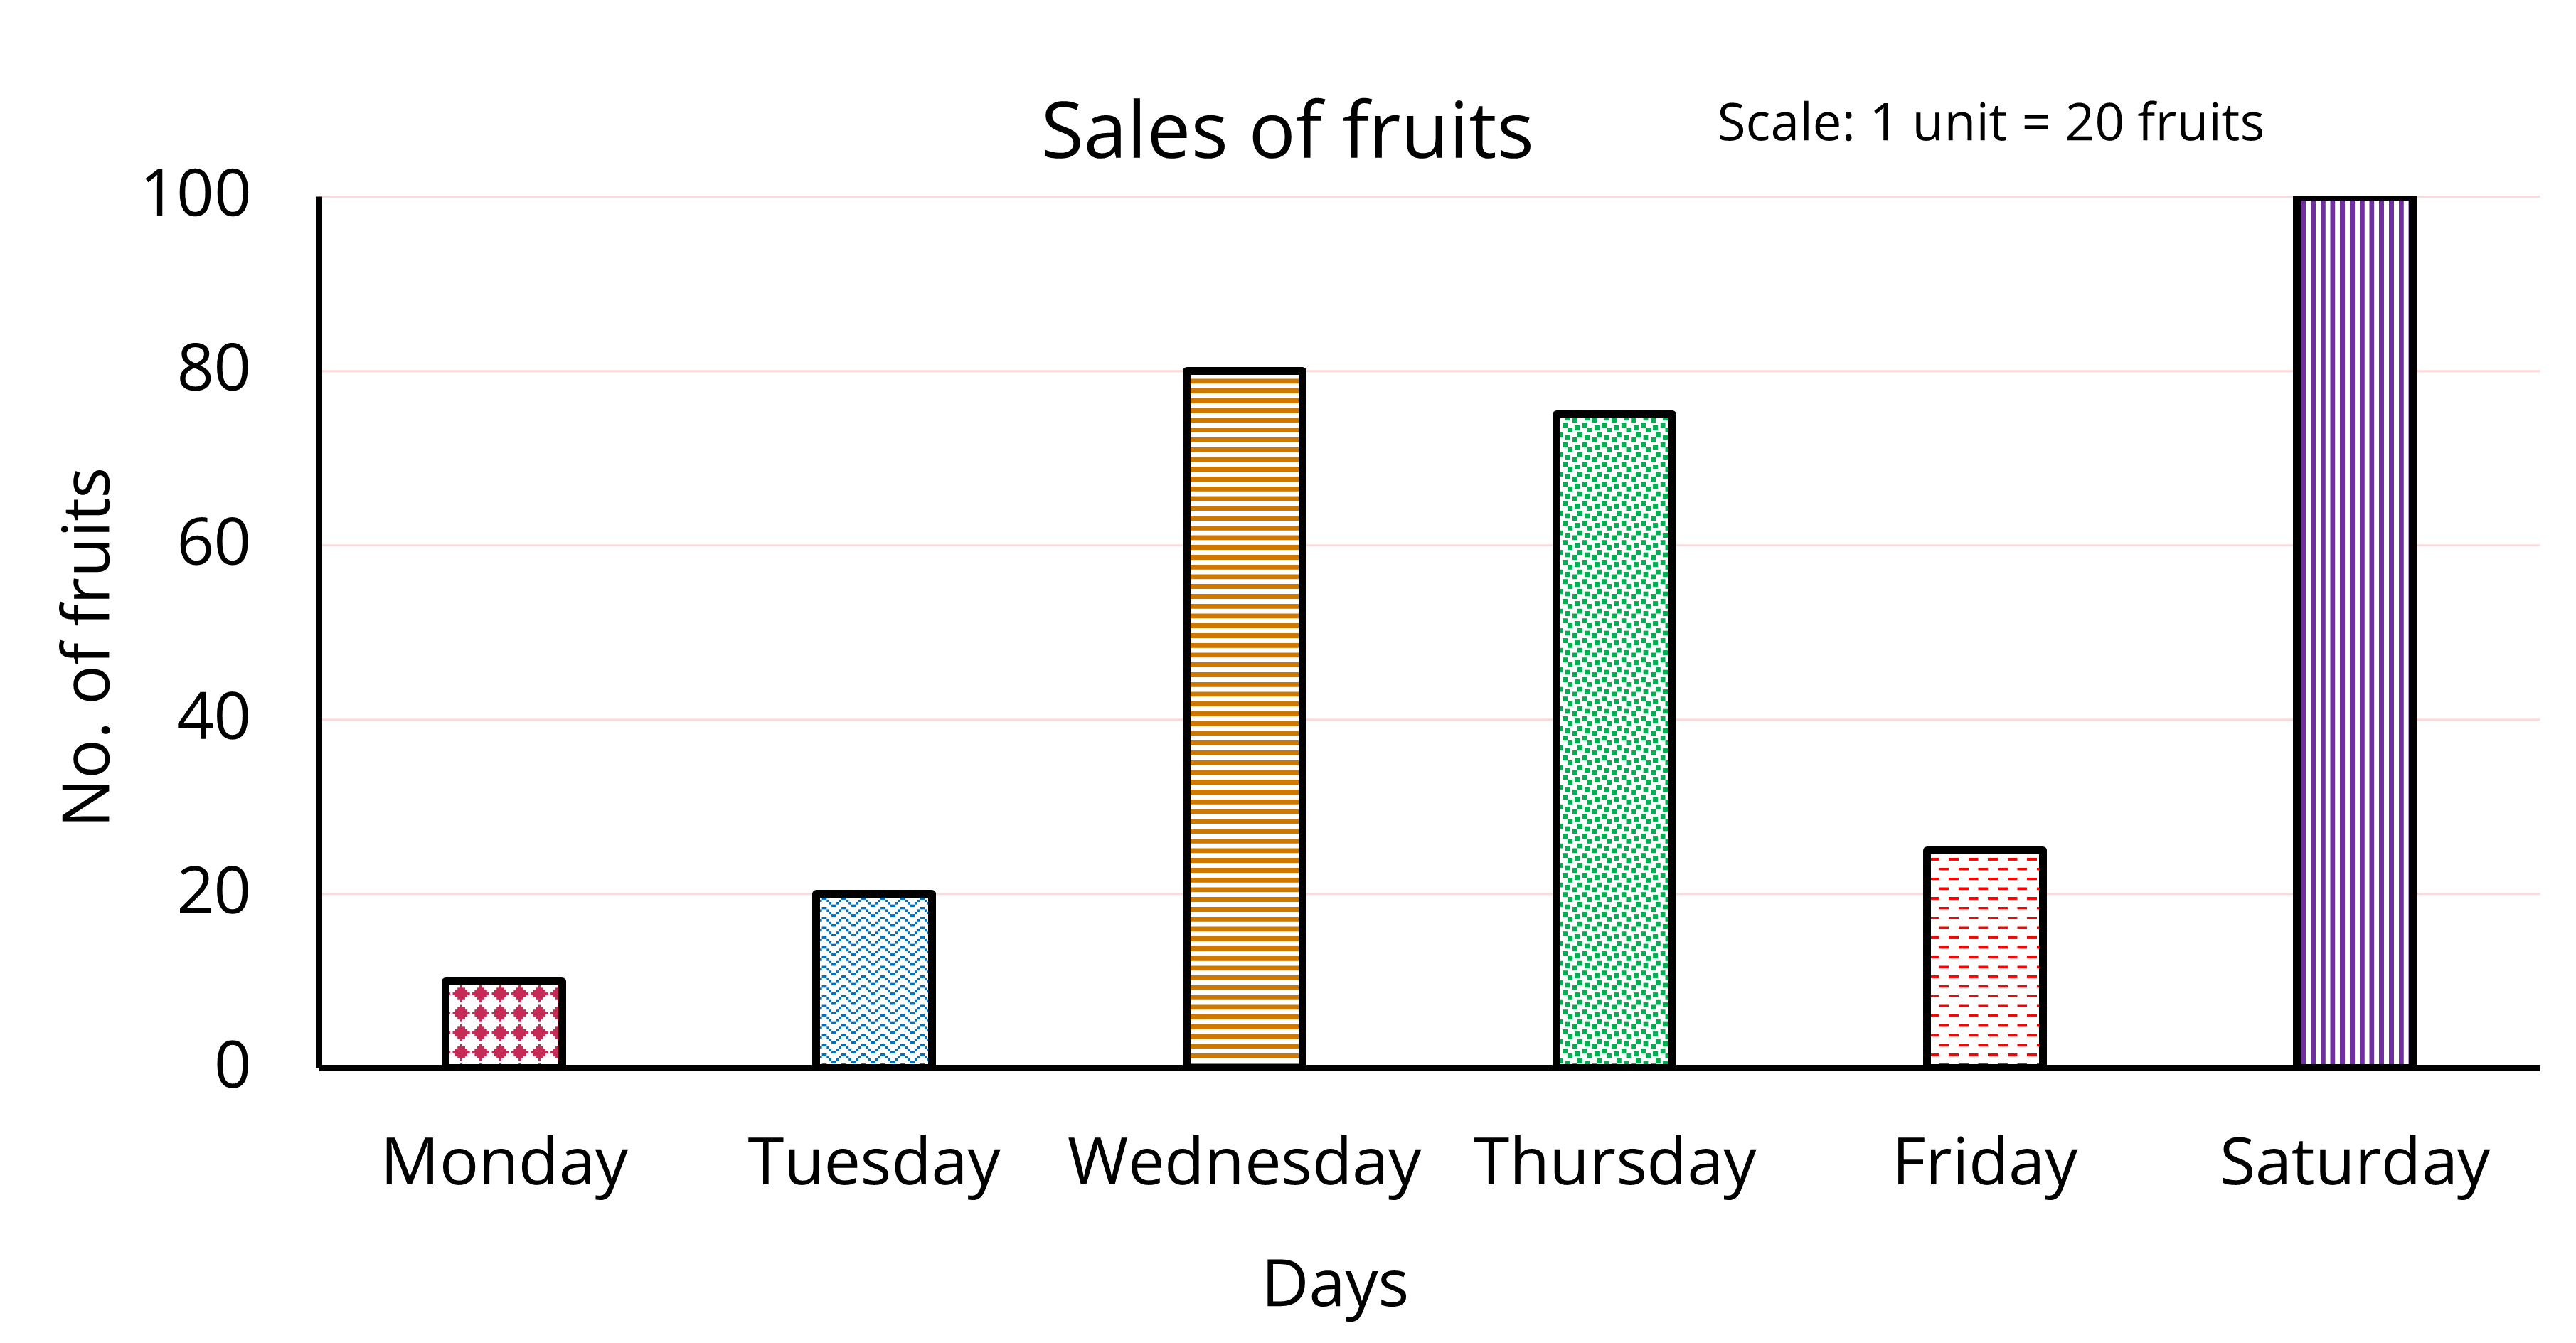
\includegraphics[width=13cm, height=6.5cm]{C6M17 - DT - Q3.png}},
optionA={Monday},
optionB={Wednesday},
optionC={Friday},
optionD={Saturday},
leftmini={0.65},
rightmini={0.25},
correctoption={A},
}

\smallskip\centering
            \renewcommand{\arraystretch}{1.25}
            \begin{tabular}{|M{2cm}|M{1cm}|M{1cm}|M{1cm}|M{1cm}|M{1cm}|}
            \hline
Option & \cellcolor{cellgreen} A (\ding{51}) & B (\ding{55}) & C (\ding{55}) & D (\ding{55}) & E\\  
\hline
5 A & \highgreen{82\%} & \highno{0\%} & \highno{0\%} & \highno{18\%} & \highno{0\%} \\            \hline
\end{tabular}

\end{minipage}

\bigskip


\begin{minipage}{\linewidth}\mcqimgleftFourOne{
questionnumber={34}, 
questiontext={Observe the given pictograph and find the number of roses sold on Thursday.},
imgtabletikz  = {
\renewcommand{\arraystretch}{1.25}
\begin{tabular}{|c|c|}
\hline
  Days & Number of roses sold (1 \smiley = 1 rose)  \\
  \hline
  Monday& \smiley \smiley \smiley  \\
  \hline
  Tuesday  & \smiley \smiley \smiley \smiley \smiley \smiley \smiley  \\
  \hline
  Wednesday & \smiley \smiley \smiley \smiley \smiley \smiley \smiley \smiley \\
  \hline
  Thursday & \smiley \smiley \smiley \smiley \smiley \smiley \\
  \hline
\end{tabular}  },
optionA={0},
optionB={8},
optionC={6},
optionD={7},
questionTag={C6M17 - DT - Q2}, 
leftmini={0.5},
rightmini={0.3},
correctoption={C},
}

\smallskip\centering
            \renewcommand{\arraystretch}{1.25}
            \begin{tabular}{|M{2cm}|M{1cm}|M{1cm}|M{1cm}|M{1cm}|M{1cm}|}
            \hline
Option & A (\ding{55}) & B (\ding{55}) & \cellcolor{cellgreen} C (\ding{51}) & D (\ding{55}) & E\\  
\hline
5 A & \highno{0\%} & \highno{0\%} & \highgreen{94\%} & \highno{6\%} & \highno{0\%} \\            \hline
\end{tabular}

\end{minipage}

\bigskip%
\end{document}